\subsection{Multijet Background Estimation}
\label{sec:multijet_background}
As discussed above, the SM backgrounds are estimated from Monte-Carlo simulation and constrained in the dedicated control regions. However, the multijet processes is poorly modelled in MC simulation due to the lack of understanding of QCD, so simulation is not feasible for this background contribution. Its contribution is from the following sources:
\begin{itemize}
	\item {\bf Photon Conversion}: When photons are travelling through detector material, the interaction between photons and nucleus induces the pair production which has the products of a electron-position pair. The electrons from this source are difficult to distinguish from the signal ones decayed from Z bosons. This contribution is considered only in the electron channel.
	\item {\bf Lepton Misidentification}: Soft charged hadrons could be blocked at ECAL and leave no signature in HCAL, which is identical to electron signatures. In this case, they are reconstructed as electrons instead of jets. This source only contributes to electron channel.
	\item {\bf Heavy Hadron Decay}: The decay products of heavy hadrons also include leptons. If their decay is close to the primary vertex, the decayed leptons are not distinguishable from the prompt ones. Both electrons and muons have the contribution from this source. 
\end{itemize}
\noindent
This background contribution is only considered in resolved channel, while it is negligible in boosted channel.\cite{EXOT-2016-28}. Different from the SM background, the multijet background estimation is performed with fake factor method, a data-driven approach. The details of this method can be found in the ATLAS Run2 VHbb analysis~\cite{ATLAS-CONF-2016-091, ATL-COM-PHYS-2016-429}. 
\\
\\{\bf Methodology}
\begin{figure}[ht]
	\centering
	\includegraphics[width=0.8\textwidth]{Chapter3/ABCD.png}
	\caption{The illustration of ABCD method with two uncorrelated parameters, A and B, to divide events into four categories, A, B, C, and D, and A is the signal/control region.}
	\label{Fig:ABCD}
\end{figure}
\\
\\The fake factor method is one type of ABCD methods with an illustration in Fig.~\ref{Fig:ABCD}. Two uncorrelated parameters are chosen to divide the data events into four categories, A, B, C, and D which are orthogonal to each other, and A is taken as the signal or control region. If the event contributions are the same across all the regions, the following equation should be held true:
\begin{equation}
\label{eq:ABCD}
\frac{N_A}{N_B} = \frac{N_C}{N_D}
\end{equation}
N stands for the event numbers in each region. With a proper choice on the parameter A and parameter B, the multijet events are enriched in region B, C, and D, and the multijet contribution in region A could then therefore be estimated with the equation shown above. The ratio of event numbers of C and D regions is called ``fake factor''.
\\
\\In this analysis, the number of small R jets is taken as parameter B, while the muon isolation (electron identification) is chosen to be parameter A for the muon (electron) channel. The fake factors are estimated from data in the region with only one small R jet selected called single jet control region (region C+ region D) which is orthogonal to signal regions which demands two or more jets. The events with any existence of fat jets passing the selection is vetoed ($p_{T}^{J}>200~GeV$ \&\& $m^{J}>50~GeV$) to keep the orthogonality to boosted regions. This region is then further divided into two subregions by muon isolation and electron identification. The first subregion has the same lepton selection as the signal region with signal leptons, while the second one has the inverse requirement on leptons with inverse leptons. The lepton definition could be seen in table \ref{tab:LepIsoCR}. With $p_{T}(\mu\nu)<150~GeV$, an isolated muon trigger is applied with a requirement on isolation of $ptvarcone30/p^{\mu}_{T}<0.07$. In this case, the isolation requirement for inverse muons is tightened to the same upper limit to keep the consistency of muons reconstructed at trigger and offline levels. $E_{T}^{miss}$ triggers instead of muon triggers are applied in the region of $p_{T}(\mu\nu)>150 GeV$, so the isolation issue is not present. Therefore, the isolation upper limit is loosen to 0.15. Then, the fake factor is defined as the ratio of event numbers of these two subregions:
\begin{equation}
\label{eq:ff}
 f = \frac{N_{event}(CR(1j, \ell\left[signal\right]))}{N_{event}(CR(1j, \ell\left[inverse\right]))}
\end{equation}
Furthermore, to achieve a better accuracy, this was performed in the binnings presented in Tab.~\ref{tab:FFBinning}. The fake factors have the dependence on lepton $\eta$ (this dependence is for the consideration of detector homogeneity) and lepton $p_{T}$ (the multijet background contribution source varies with lepton $p_{T}$). Additional binning on the $E_{T}^{miss}$ is applied in electron channel. For both channels, the fake factor is estimated in two different regions with $p_{T}(\mu\nu)<150~GeV$ and $p_{T}(\mu\nu)>150~GeV$, because they have different amount of multijet contamination. Fake factors are shown as a function of lepton $p_{T}$ in Figure~\ref{fig:fakefactor} for the region of $p_{T}(l\nu)>150~GeV$ for which it could be noticed that fake factors for electron channel are just up to $p_{T}=190~GeV$. To have the multijet background estimation for high $p_T$ electrons with $p_{T}>190~GeV$, fake factors are roughly evaluated in $p_{T}$ bins only for this $p_T$ range which is shown in Fig.~\ref{fig:fakefactor_el_highPt}.
\begin{table}[h]
  \caption{Definition of leptons in the single jet control regions} \label{tab:LepIsoCR}
  \begin{center}

    \begin{tabular}{ | c | c | c | }
     \hline
                               &  Signal Lepton  & Inverse Lepton \\ \hline
    electron                   &        TightLH        & MediumLH (!TightLH) \\ \hline
    muon($p_{T}(l\nu)>150 GeV$) &  $Iso_{trk}<0.06$    & $0.06<Iso_{trk}<0.15$ \\ \hline
    muon($p_{T}(l\nu)<150 GeV$) &  $Iso_{trk}<0.06$    & $0.06<Iso_{trk}<0.07$ \\ \hline
\end{tabular}
\end{center}
\end{table}


\begin{table}[h]
  \caption{Binning for electrons and muons to evaluate fake factor} \label{tab:FFBinning}
\begin{center}

\begin{tabular}{ | c | c | c | c |}
    \hline
    channel  & $p_{T}(GeV)$ & $|\eta|$ & $E_{T}^{miss}(GeV)$ \\ \hline
    electron & 27-115 &  & 0, 60, 75, $\infty$ \\
             & 115-135&0, 1.37, 1.52, 2.47 & 0, 38, 52, $\infty$ \\
             & 135-155& & 0, 26, 43, $\infty$ \\
             & 155-190& & 0, 25, 45, $\infty$ \\ \cline{2-4}
             & Fig.~\ref{fig:fakefactor_el_highPt} (190-$\infty$) & NA & NA  \\\hline
    muon     & 27, 42, 59, 76, 99, $\infty$ & 0, 1.05, 1.5, 2.5 & N/A \\ \hline

\end{tabular}
\end{center}
\end{table}

\begin{figure}[ht]
       \centering
       \subfloat[]{\includegraphics[width=0.45\textwidth]{Chapter3/fakefactor_el_medium_highpTW}}
       \subfloat[]{\includegraphics[width=0.45\textwidth]{Chapter3/fakerate_mu_ewk}} \\
       \caption{Fake factors for the corresponding binnings (shown in text) in electron (a) and muon (b) channels}
       \label{fig:fakefactor}
\end{figure}

\begin{figure}[ht]
       \centering
       \subfloat[]{\includegraphics[width=0.45\textwidth]{Chapter3/fakerate_el_highPt.pdf}}
       \caption{Fake factors for high $p_T$ electrons}
       \label{fig:fakefactor_el_highPt}
\end{figure}
\noindent
The fake factors are then applied on events from the ``inverse leptopn'' control regions. They have the same event selection as the signal and control regions, but the only lepton in those events is required to be an inverse leptons with the same definition as shown in Tab.~\ref{tab:LepIsoCR} (Region B in Fig.~\ref{Fig:ABCD}). With Eq.~\ref{eq:ABCD}, it could be seen that the multijet event number in the region of interest ($N_A$) could be presented as:
\begin{equation}
N_A = N_B \times f
\end{equation}
with f from Eq.~\ref{eq:ff}. Therefore, fake factors could be used as event weights applied on events from inverse lepton control regions, which then gives the multijet event number in the signal/control regions. 
\subsubsection*{Electroweak Subtraction}
Electroweak interactions ($t\bar{t}$, W/Z+jets, diboson and single top) could also contribute to multijet events in addition to the multijet background, so they might be double counted from the fake factor method and background simulation. To avoid this issue, those events are removed by employing fake factors on events from the simulation in the inverse lepton control region, which could be expressed as the following equation:
\begin{equation}
 N^{MJ}_{events} = N^{data}_{events}-N^{MC}_{event}
\end{equation}
It means that the multijet background events ($N^{MJ}_{events}$) are given by removing the estimated SM multijet contribiton (from simulation) ($N^{MC}_{event}$) from the estimated multijet events (from data)($N^{data}_{events}$), and it is anticipated that $N^{data}_{events}\approx N^{MC}_{event}$ with $E^{miss}_{T}>150~GeV$. A control region was defined to verify this with a simple selection of at least two small-R jets with $p_{T}>20~GeV$ and exactly one signal electron or muon. This region is overlapped with signal regions, while the signal events just account for a small fraction, so this doesn't bias the final result. The comparison between data and the SM background from the MC simulation in this control region is shown in Figure~\ref{fig:dijetFakeCR_el} and Figure~\ref{fig:dijetFakeCR_mu} for electron and muon channels respectively. The observed discrepancy was contributed by the multijet events. However, unfortunately, an inconsistency remains in the region of $E_{T}^{miss}>150~GeV$. That means the multijet events from the SM backgrounds (electroweak interactions) are not well-modelled. In this case, the electroweak subtraction is applied with a scale factor derived from the ratio of events from data and simulation in the bin of $150 GeV<E^{miss}_{T}<250~GeV$ defined as: 
\begin{equation}
f = \frac{N_{event}(data)}{N_{event}(MC)}
\end{equation}
It is applied as an additional correction on fake factors for events with $E_{T}^{miss}>150 GeV$ from simulation to correct this MC mis-modelling. The electroweak subtraction factors for electron and muon channels are shown in Tab~\ref{tab:ewsubtraction}. For the $\met<150~GeV$ region, the simulation sample has the performance as what we expected, so this correction is not applied. 

\begin{figure}[ht]
       \centering
       \subfloat[]{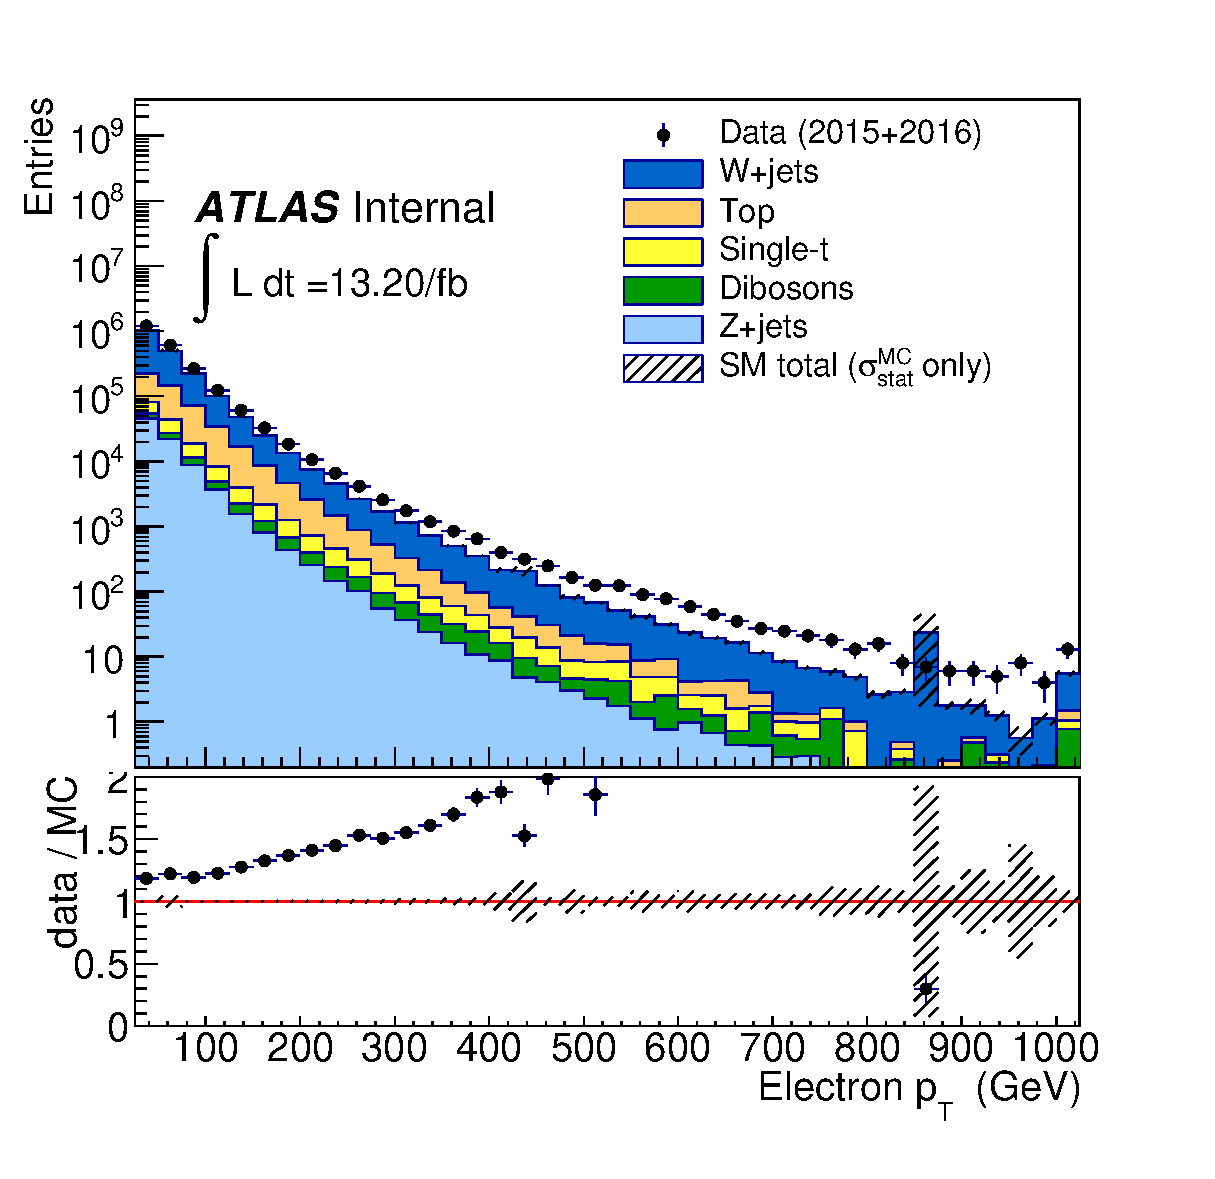
\includegraphics[width=0.45\textwidth]{Chapter3/MJ_CR/electronPt.eps}}
       \subfloat[]{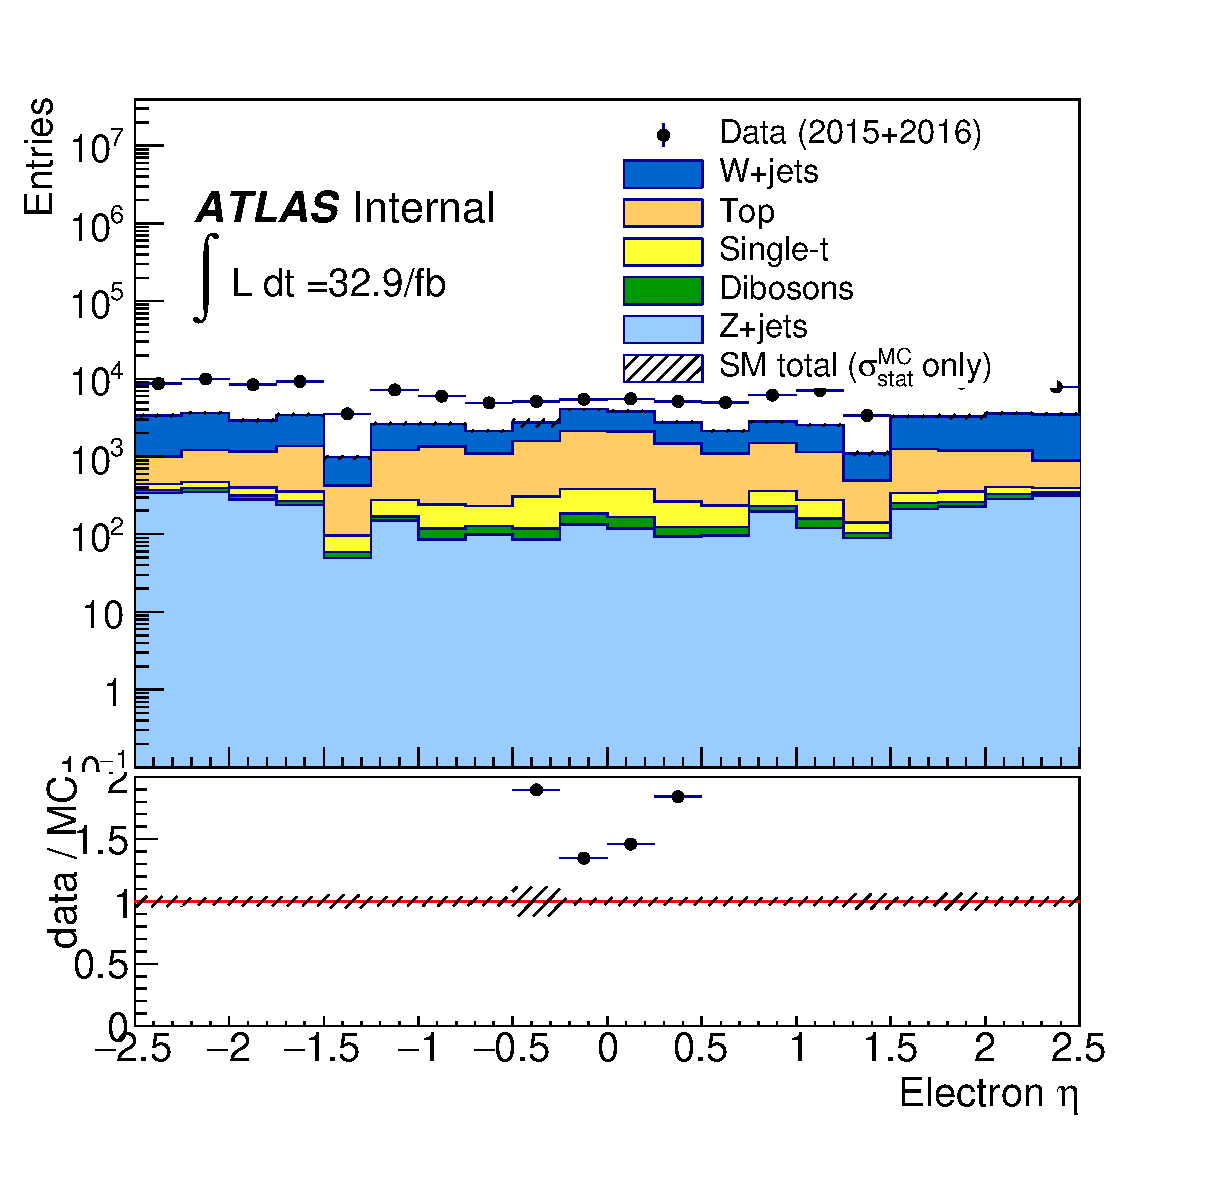
\includegraphics[width=0.45\textwidth]{Chapter3/MJ_CR/electronEta.eps}}\\ 
       \subfloat[]{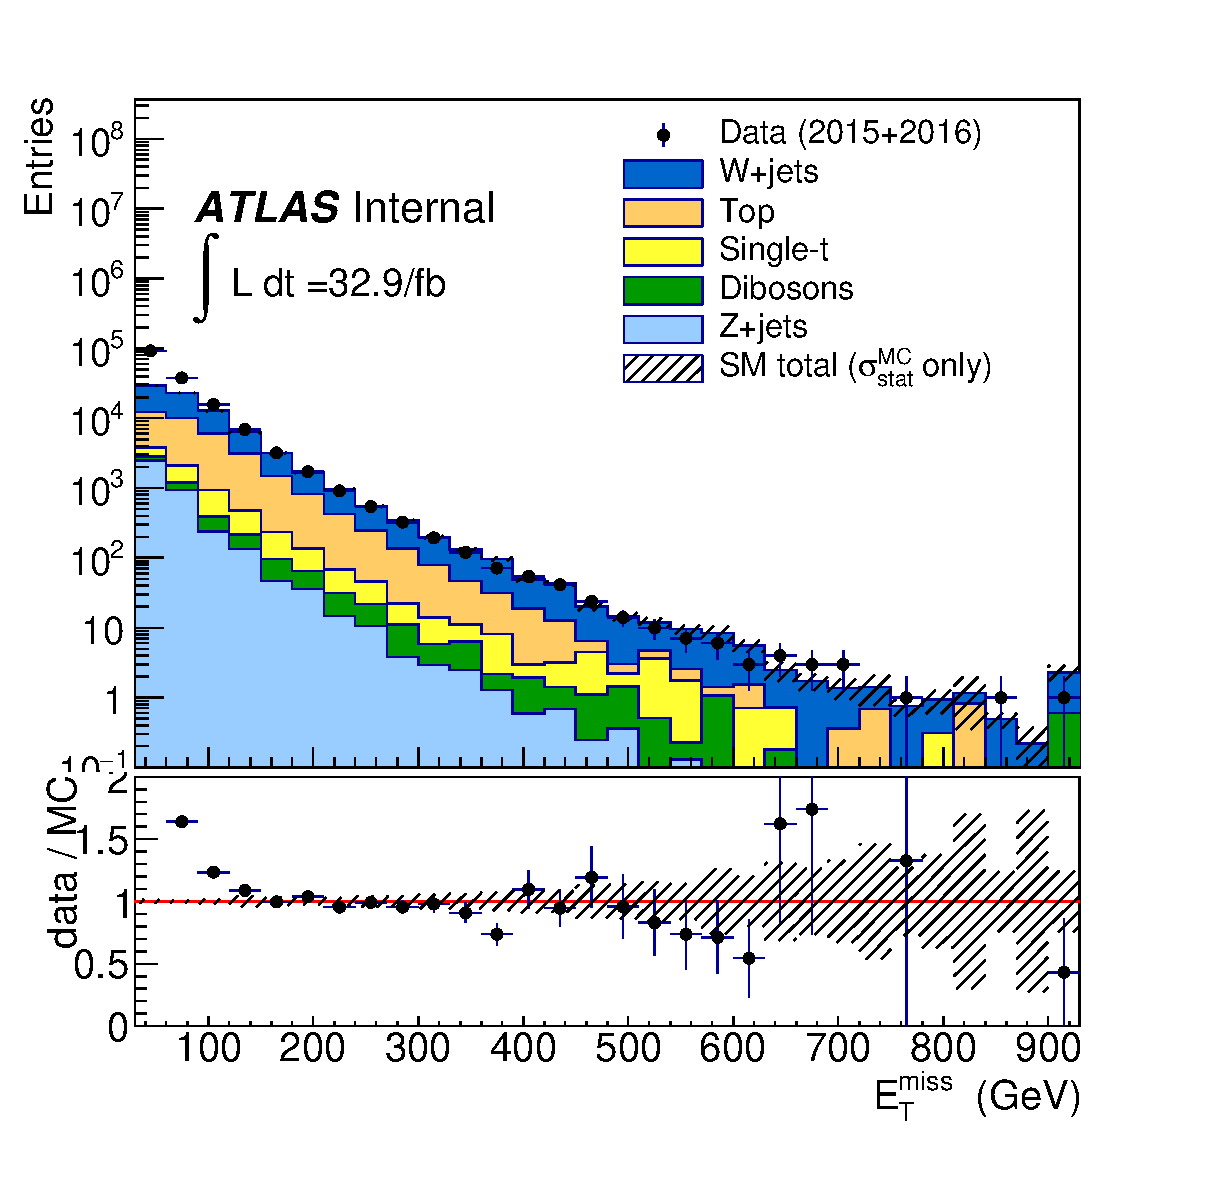
\includegraphics[width=0.45\textwidth]{Chapter3/MJ_CR/met_el.eps}}
       \subfloat[]{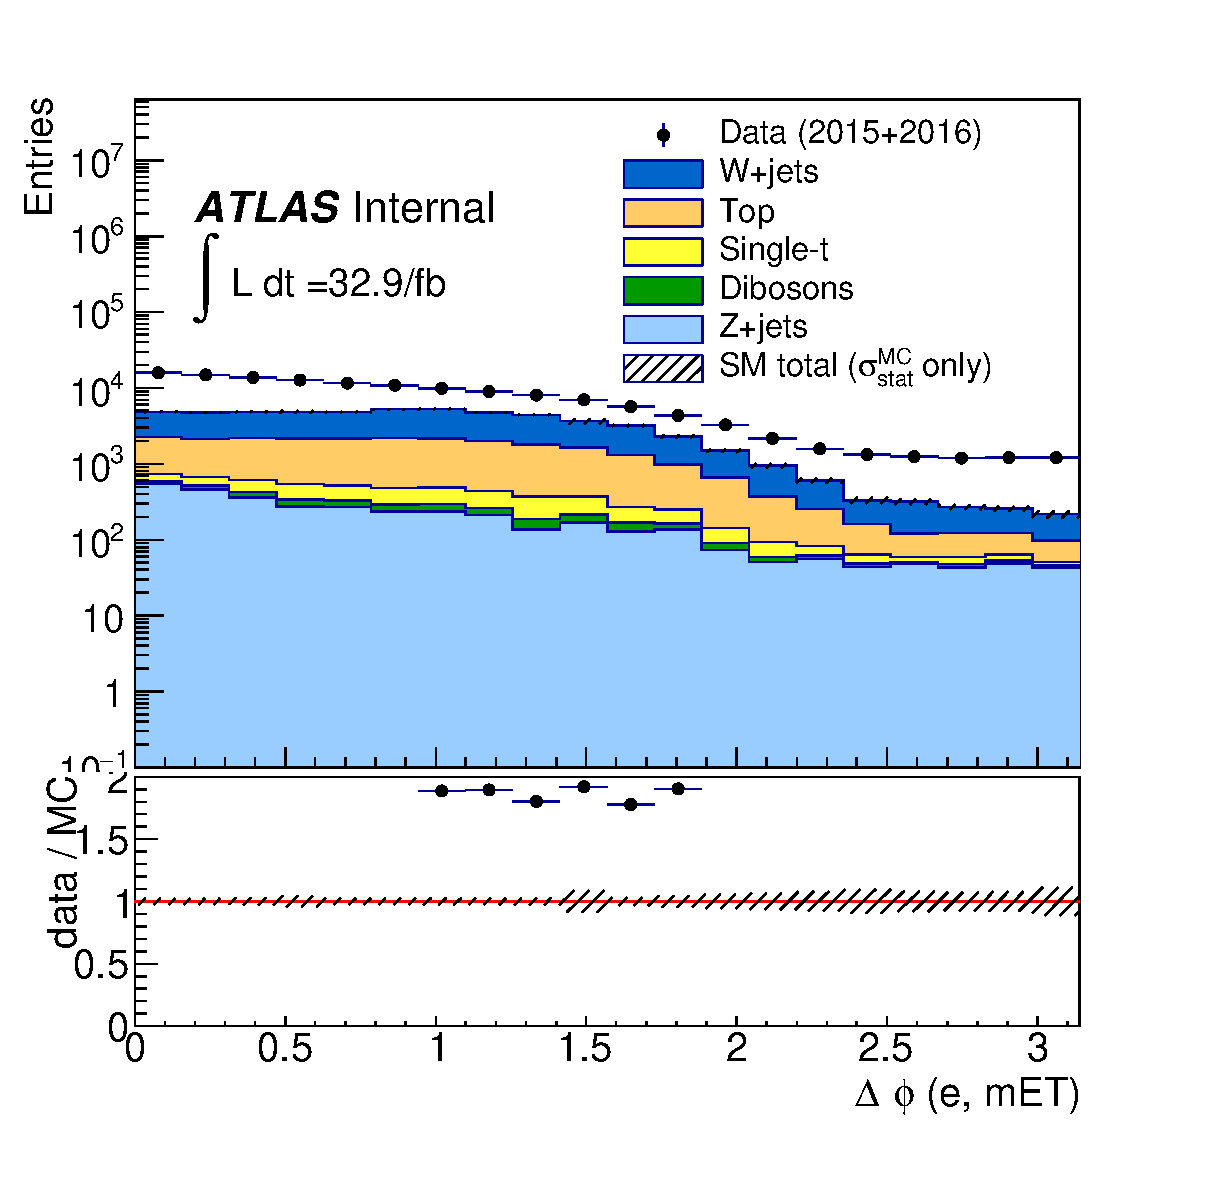
\includegraphics[width=0.45\textwidth]{Chapter3/MJ_CR/dphilepmet_el.eps}}\\
       \caption{The distribution of lepton $p_{T}$, $\eta$, $E_{T}^{miss}$ and $\Delta\phi$(e,$E_{T}^{miss}$) in dijet fake control region with inversed lepton for electron channel. The inconsistency is thought to be comprised of multijet events without applying electroweak subtraction.} 
       \label{fig:dijetFakeCR_el}
\end{figure}

\begin{figure}[ht]
       \centering
       \subfloat[]{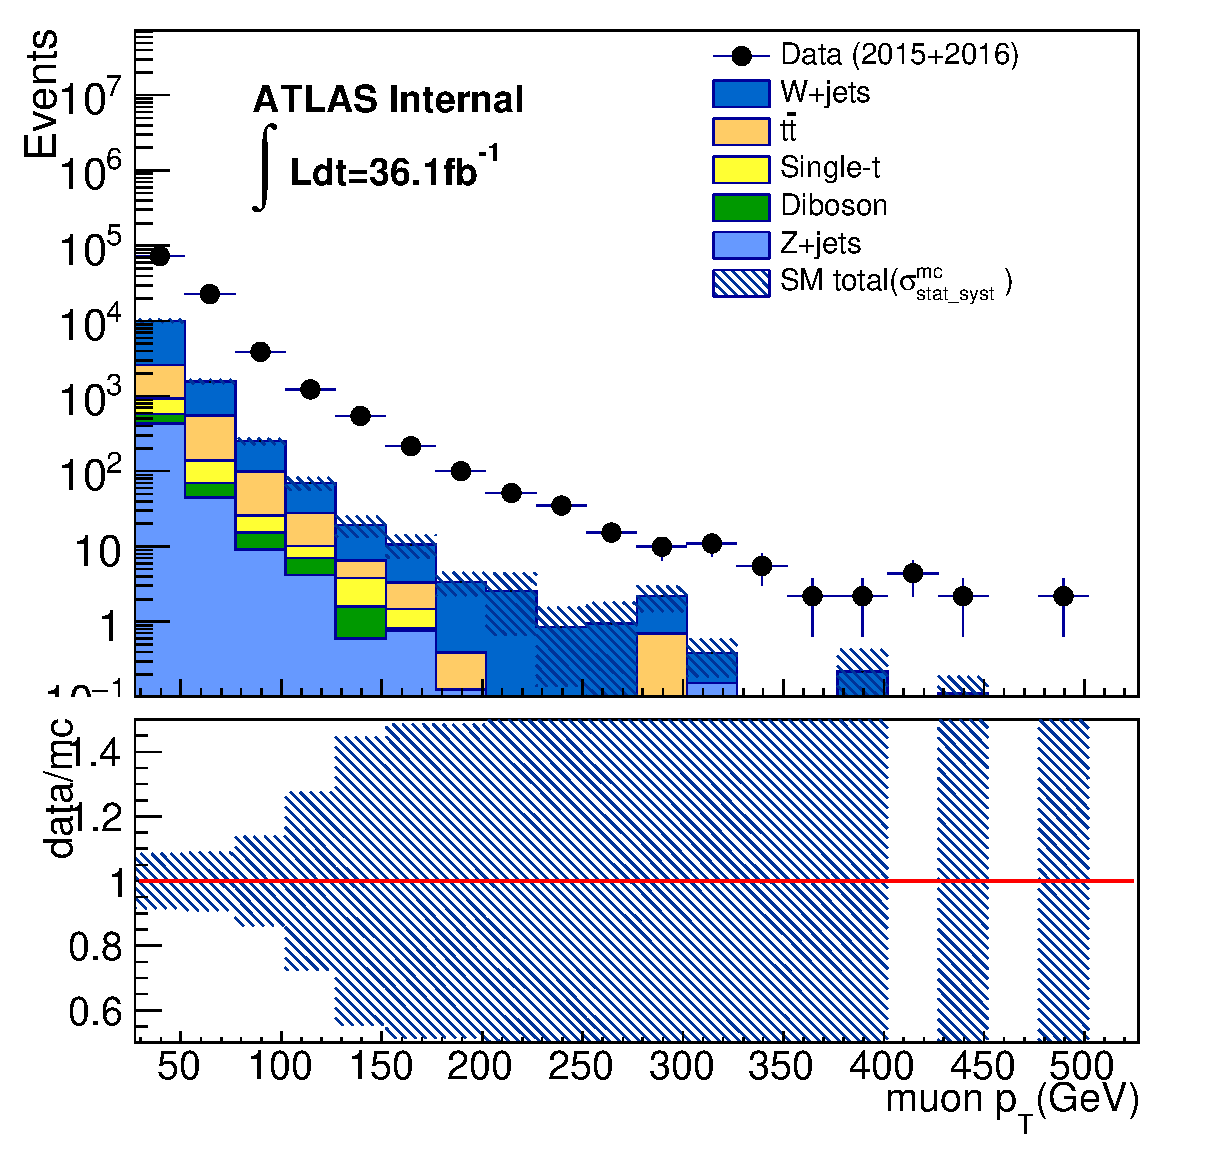
\includegraphics[width=0.45\textwidth]{Chapter3/MJ_CR/muonPt.eps}}
       \subfloat[]{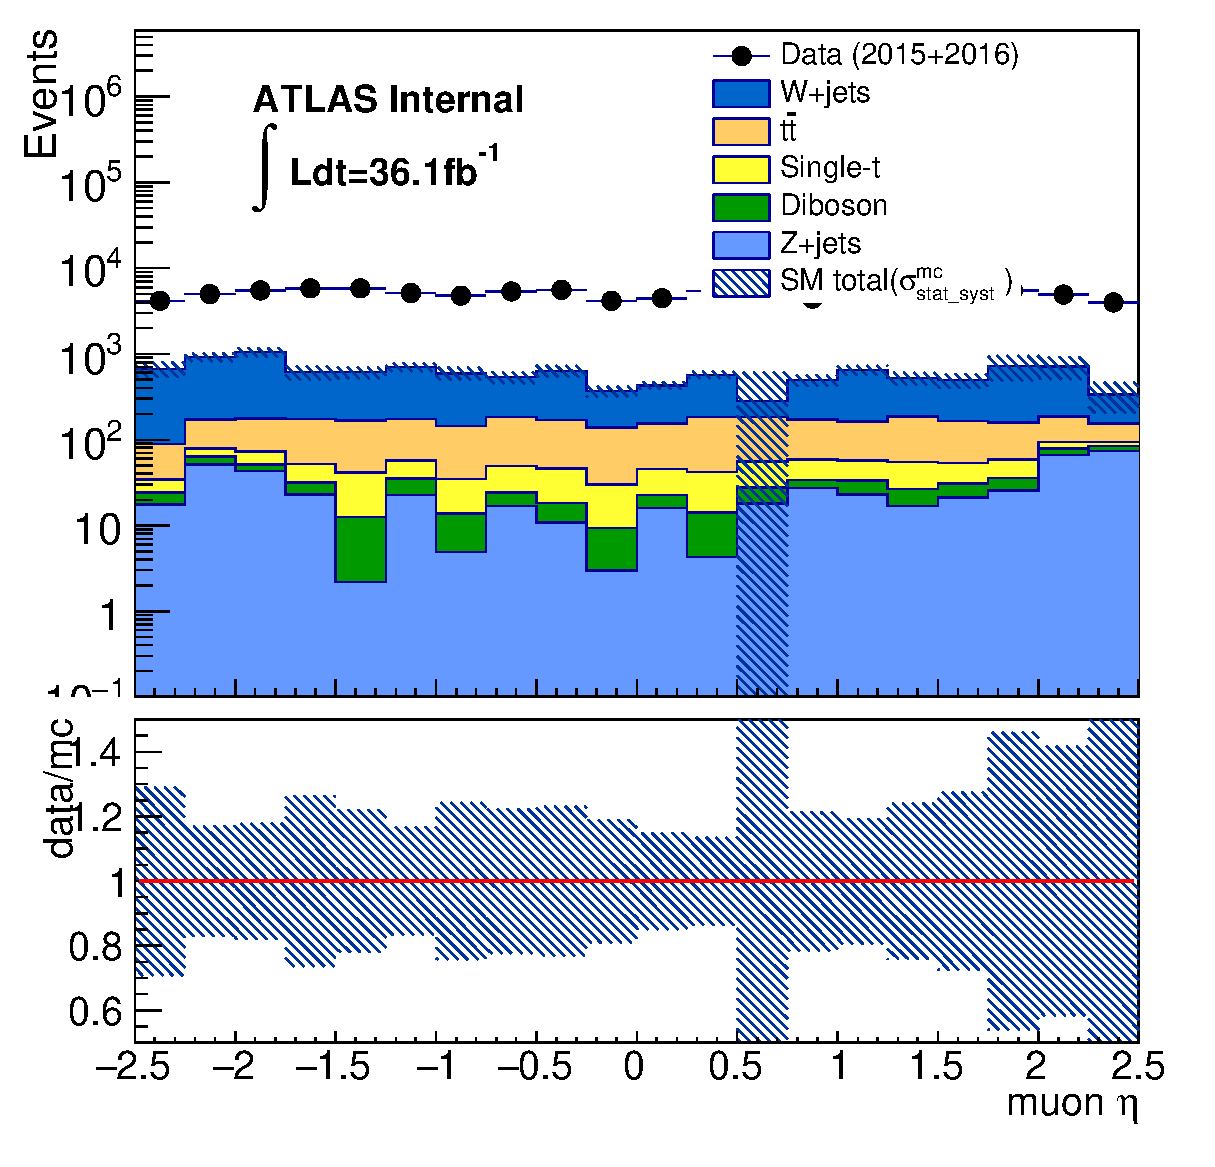
\includegraphics[width=0.45\textwidth]{Chapter3/MJ_CR/muonEta.eps}} \\
       \subfloat[]{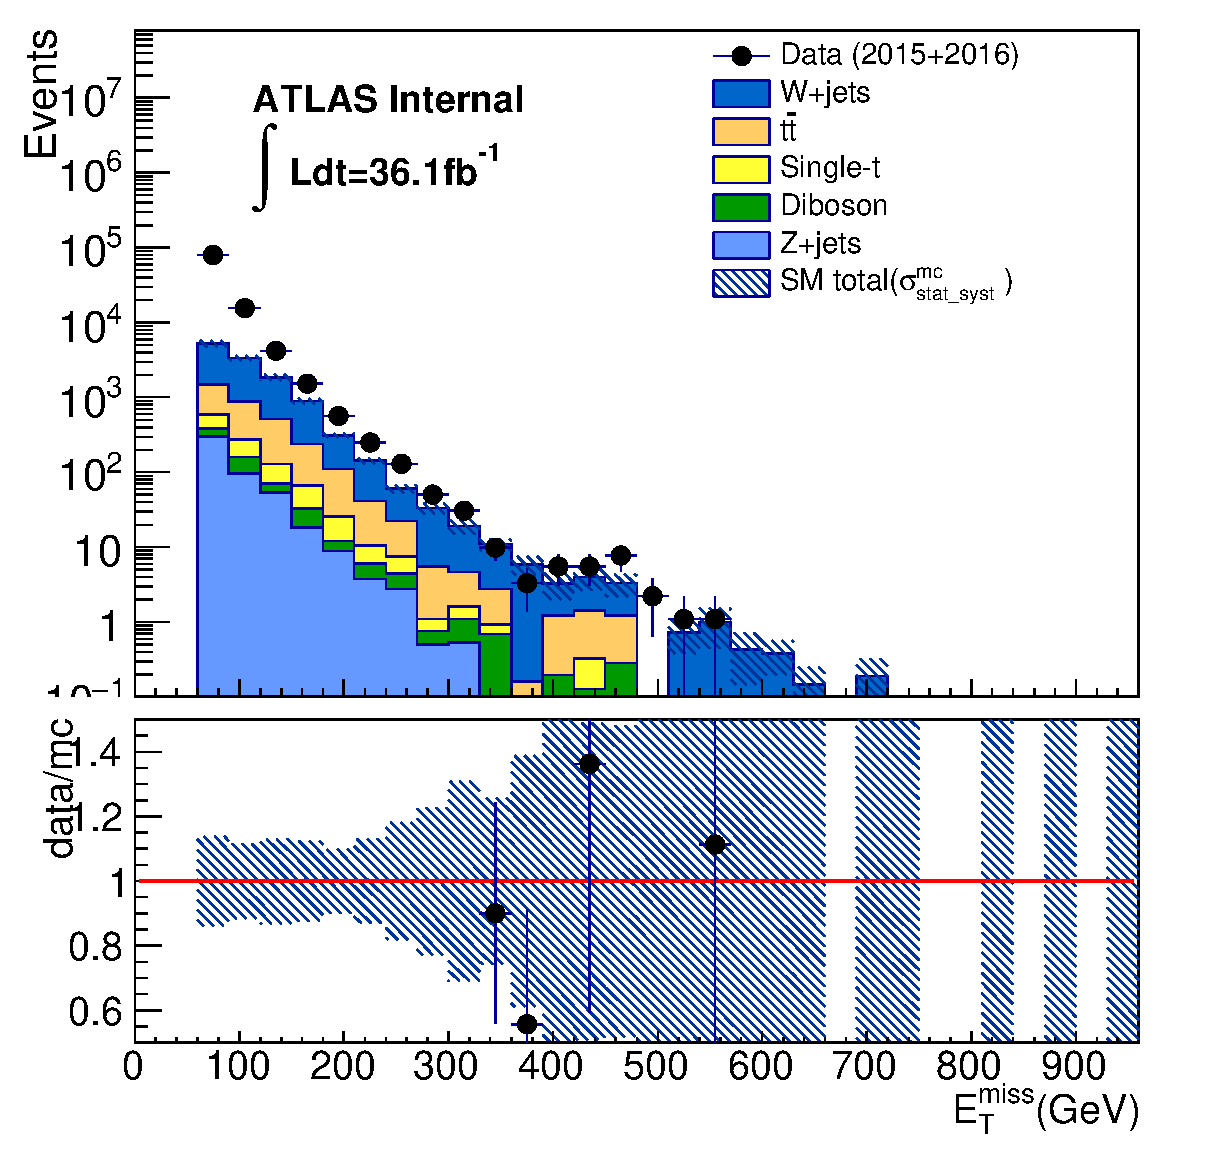
\includegraphics[width=0.45\textwidth]{Chapter3/MJ_CR/met_mu.eps}}
       \subfloat[]{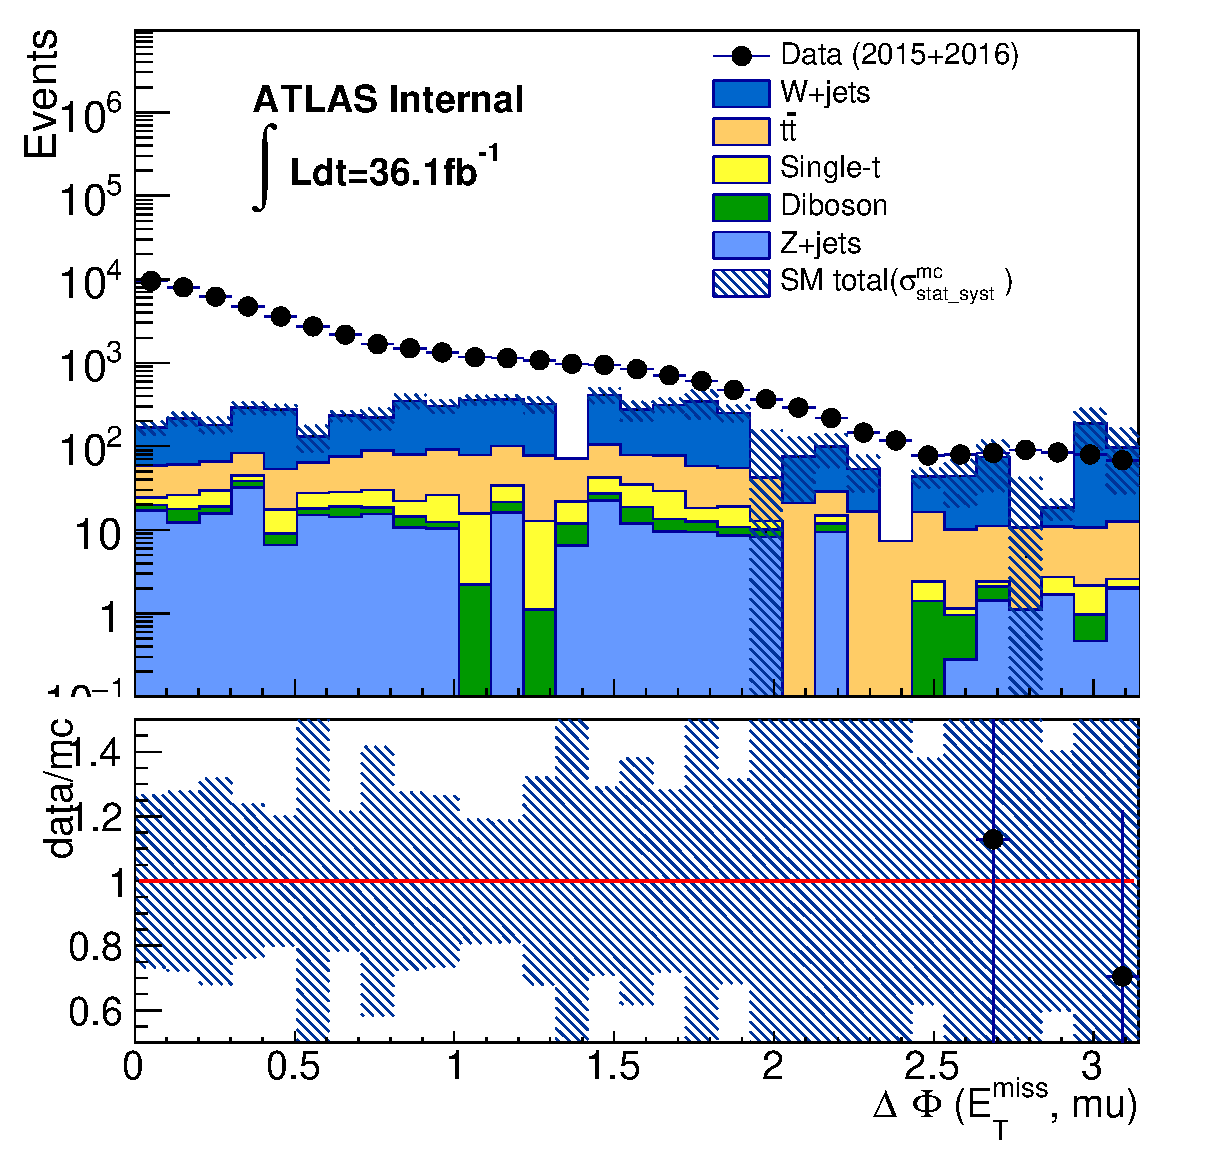
\includegraphics[width=0.45\textwidth]{Chapter3/MJ_CR/dphilepmet_mu.eps}}\\
       \caption{The distribution of lepton $p_{T}$, $\eta$, $E_{T}^{miss}$ and $\Delta\phi$($\mu$,$E_{T}^{miss}$) in dijet fake control region with inversed lepton for muon channel. The inconsistency is thought to be comprised of multijet events without applying electroweak subtraction.}
       \label{fig:dijetFakeCR_mu}
\end{figure}

\begin{table}[h]
  \caption{Electroweak subtraction factor for electron and muon channels} \label{tab:ewsubtraction}
  \begin{center}

    \begin{tabular}{ | c | c | c | }
     \hline
     channels                       &   electron   & muon \\ \hline
     EW subtraction factor          &   1.36       & 1.49 \\ \hline
\end{tabular}
\end{center}
\end{table}

\subsubsection*{Validation}
The method is validated in the dedicated validation region. The definition is similar to the signal region with looser cut to enrich the multijet events. It requires at lease two resolved jets ($p_{T}^{leading}>60~GeV$, $p_{T}^{subleading}>45~GeV$), $30~GeV<E^{miss}_{T}<100~GeV$, exactly one isolated lepton and the resolved triggers passed for electron and muon channels respectively. This definition is slightly overlapped with signal and control regions, but the upper cut on $E^{miss}_{T}$ suppress the signal contribution.  As the fake factors were derived from two bins of $p_{T}(l\nu)$, the validation is performed on $p_{T}(l\nu)<150~GeV$ and $p_{T}(l\nu)>150~GeV$ separately. The results are presented in Figures~\ref{fig:FakeVR1_el} -~\ref{fig:FakeVR2_mu} with multijet background estimated using fake factor method. In general, data agrees well with backgrounds with tolerable inconsistency within statistic uncertainties. The disagreement in the region of $p_{T}(l\nu)>150 GeV$ is supposed to be due to the low statistics for fake factor estimation in the single jet control region. This doesn't have a great impact in the final result, as multijet events would just account for around 10\% of all the background. The related systematic uncertainties will be discussed in Chapter~\ref{Ch:resonance_stat}.
\begin{figure}[ht]
	\centering
	\subfloat[]{\includegraphics[width=0.43\textwidth]{Chapter3/MJ_VR/lep1pt_Loose_el_highWpt}}
	\subfloat[]{\includegraphics[width=0.43\textwidth]{Chapter3/MJ_VR/lep1eta_Loose_el_highWpt}}\\
	\subfloat[]{\includegraphics[width=0.43\textwidth]{Chapter3/MJ_VR/met_Loose_el_highWpt}}
	\subfloat[]{\includegraphics[width=0.43\textwidth]{Chapter3/MJ_VR/dphilepmet_Loose_el_highWpt}}\\
	\subfloat[]{\includegraphics[width=0.43\textwidth]{Chapter3/MJ_VR/lvjjmass_Loose_el_highWpt}}
	\caption{The distribution of lepton $p_{T}$, $\eta$, $E_{T}^{miss}$, $\Delta\phi$($\ell$,$E_{T}^{miss}$), and $m_{WV}$ in validation region with $p_{T}(l\nu)>150 GeV$ in electron channel with multijet background}
	\label{fig:FakeVR1_el}
	
\end{figure}

\begin{figure}[ht]
	\centering
	\subfloat[]{\includegraphics[width=0.43\textwidth]{Chapter3/MJ_VR/lep1pt_Loose_el_lowWpt}}
	\subfloat[]{\includegraphics[width=0.43\textwidth]{Chapter3/MJ_VR/lep1eta_Loose_el_lowWpt}}\\
	\subfloat[]{\includegraphics[width=0.43\textwidth]{Chapter3/MJ_VR/met_Loose_el_lowWpt}}
	\subfloat[]{\includegraphics[width=0.43\textwidth]{Chapter3/MJ_VR/dphilepmet_Loose_el_lowWpt}}\\
	\subfloat[]{\includegraphics[width=0.43\textwidth]{Chapter3/MJ_VR/lvjjmass_Loose_el_lowWpt}}
	\caption{The distribution of lepton $p_{T}$, $\eta$, $E_{T}^{miss}$, $\Delta\phi$($\ell$,$E_{T}^{miss}$), and $m_{WV}$ in validation region with $p_{T}(l\nu)<150 GeV$ in electron channel with multijet background}
	\label{fig:FakeVR2_el}
\end{figure}

\begin{figure}[ht]
	\centering
	\subfloat[]{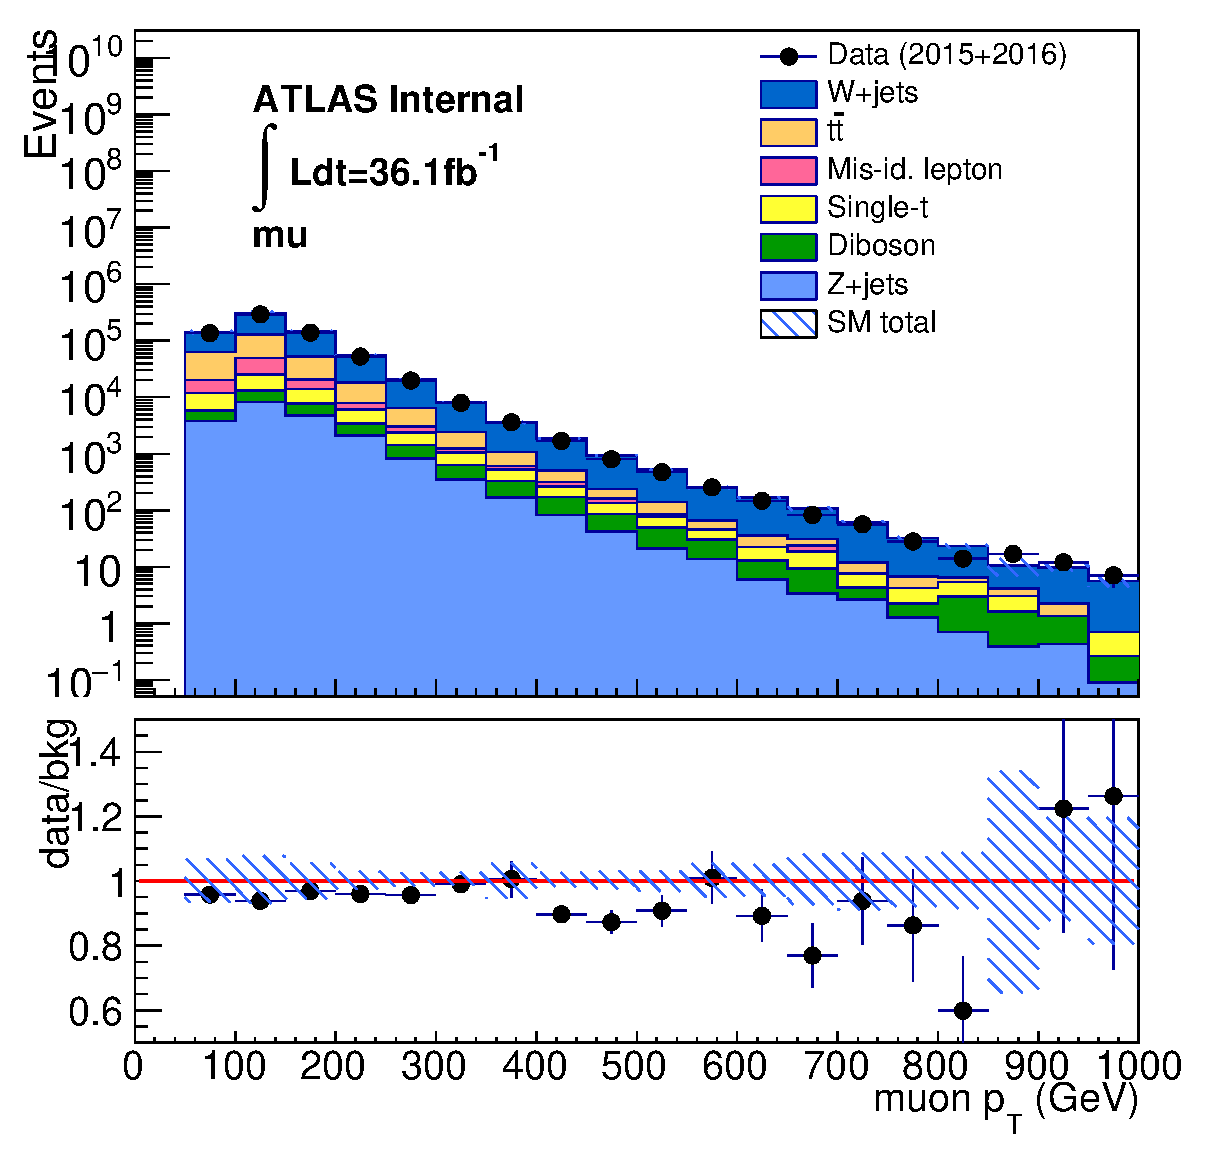
\includegraphics[width=0.43\textwidth]{Chapter3/MJ_VR/lep1pt_Loose_mu_highWpt.eps}}
	\subfloat[]{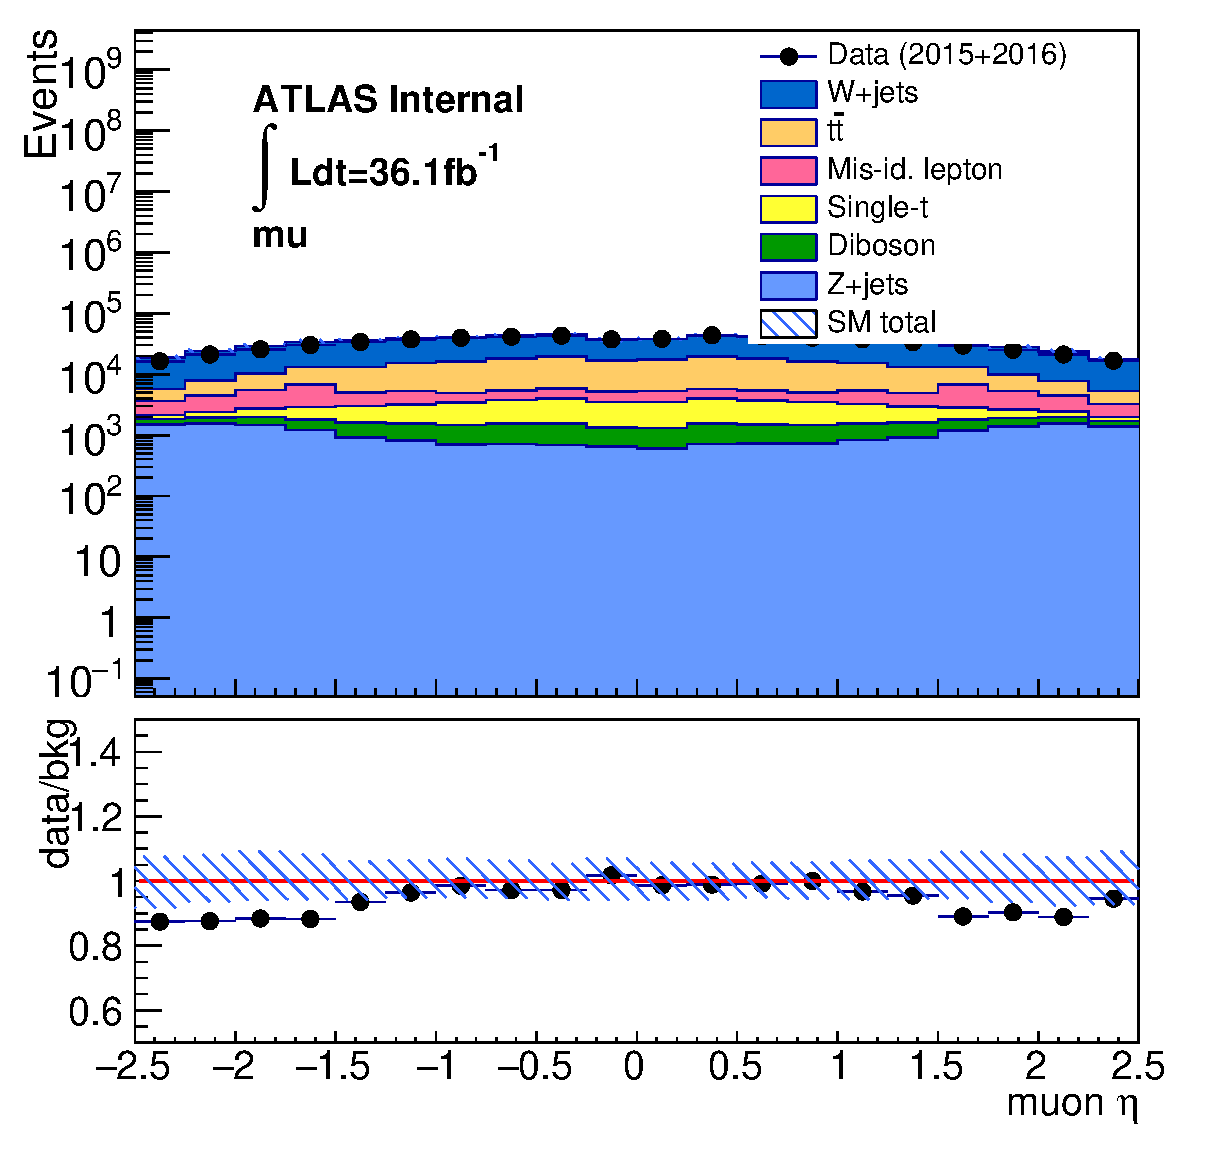
\includegraphics[width=0.43\textwidth]{Chapter3/MJ_VR/lep1eta_Loose_mu_highWpt.eps}}\\
	\subfloat[]{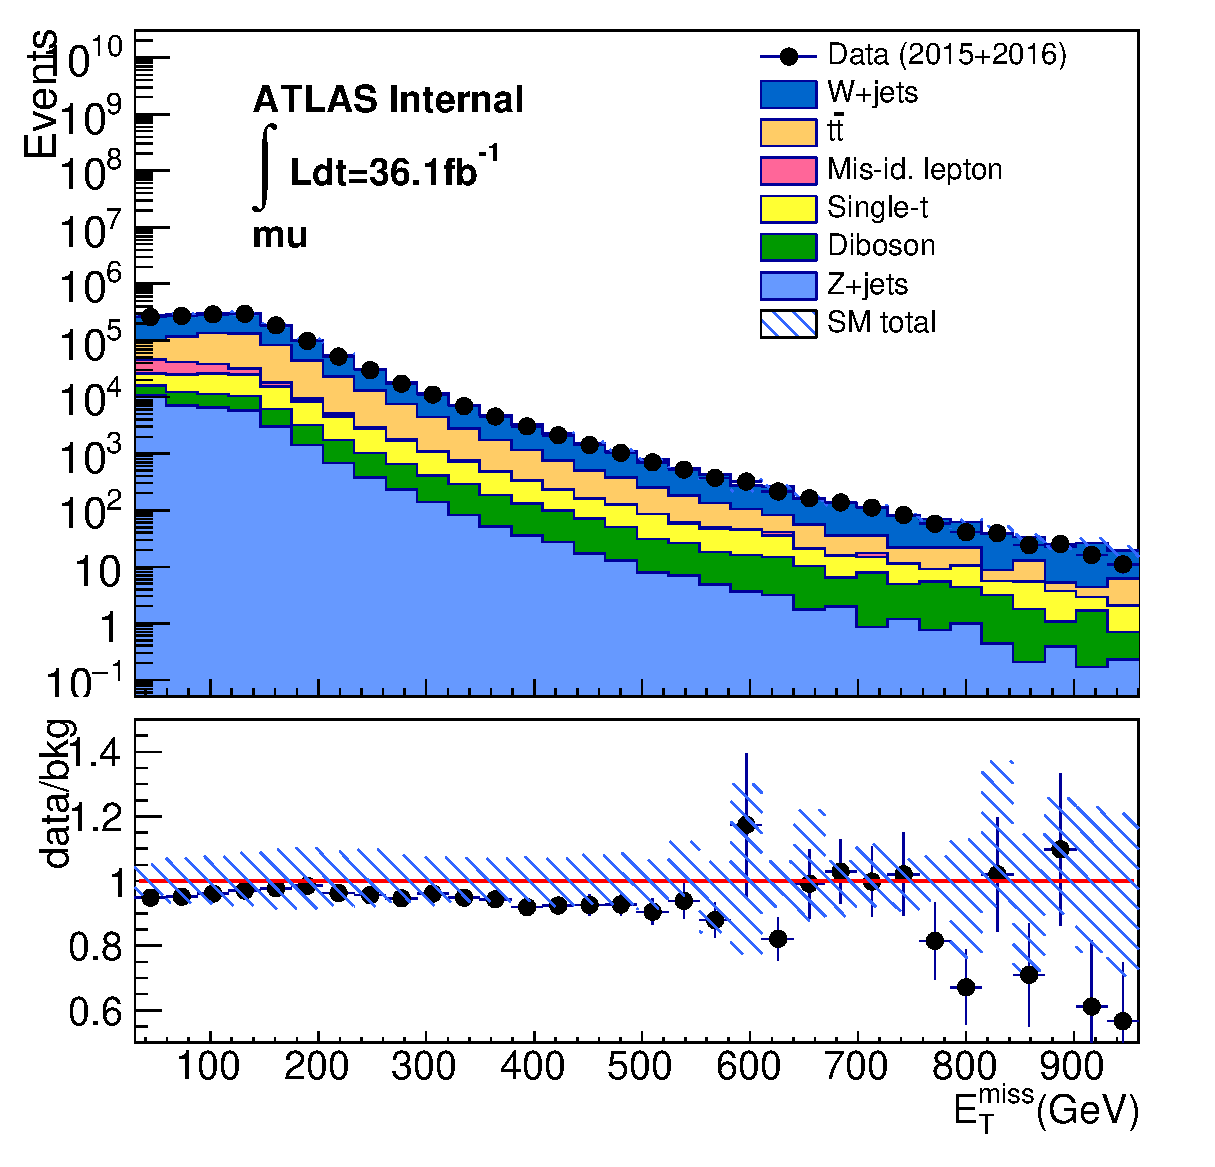
\includegraphics[width=0.43\textwidth]{Chapter3/MJ_VR/met_Loose_mu_highWpt.eps}}
	\subfloat[]{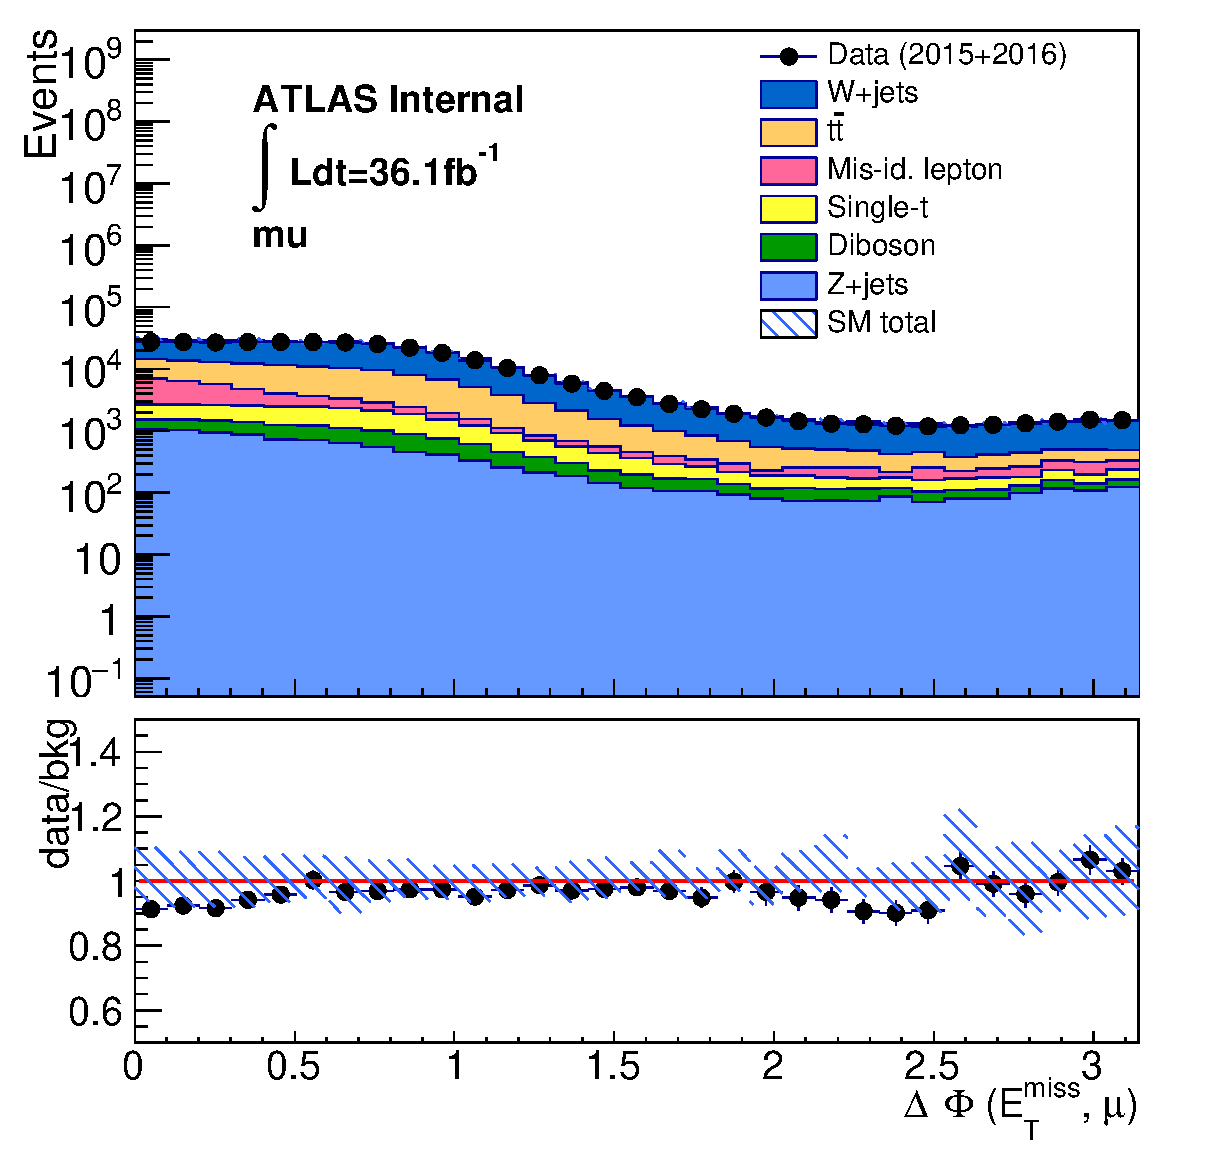
\includegraphics[width=0.43\textwidth]{Chapter3/MJ_VR/dphilepmet_Loose_mu_highWpt.eps}}\\
	\subfloat[]{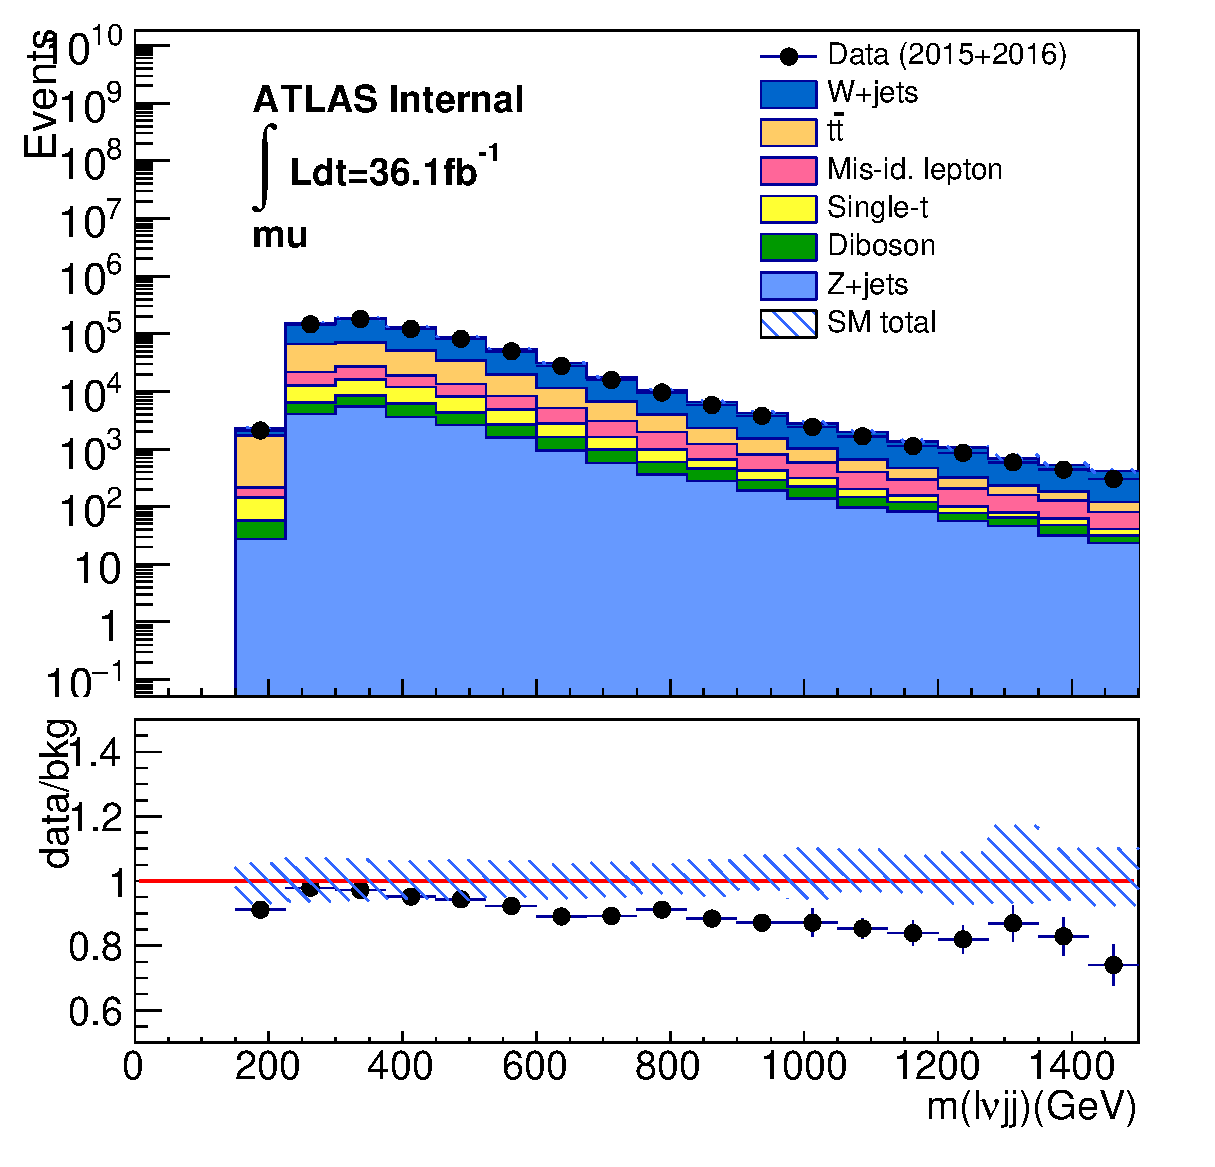
\includegraphics[width=0.43\textwidth]{Chapter3/MJ_VR/lvjjmass_Loose_mu_highWpt.eps}}
	\caption{The distribution of lepton $p_{T}$, $\eta$, $E_{T}^{miss}$, $\Delta\phi$($\ell$,$E_{T}^{miss}$), and $m_{WV}$ in validation region with $p_{T}(l\nu)>150 GeV$ in muon channel with multijet background}
	\label{fig:FakeVR1_mu}
\end{figure}

\begin{figure}[ht]
	\centering
	\subfloat[]{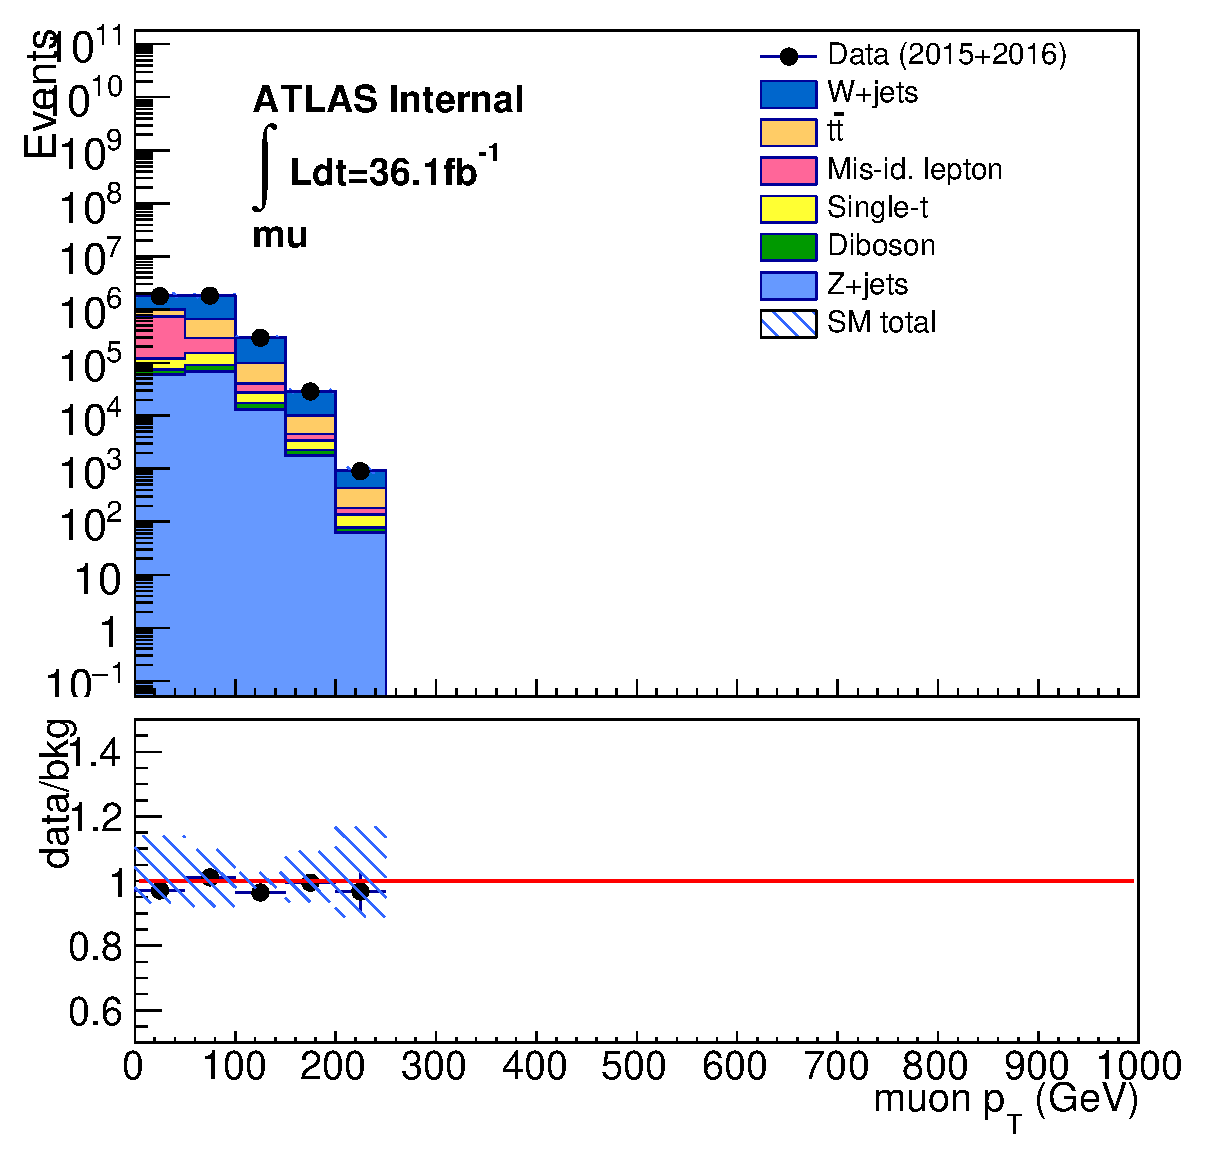
\includegraphics[width=0.43\textwidth]{Chapter3/MJ_VR/lep1pt_Loose_mu_lowWpt.eps}}
	\subfloat[]{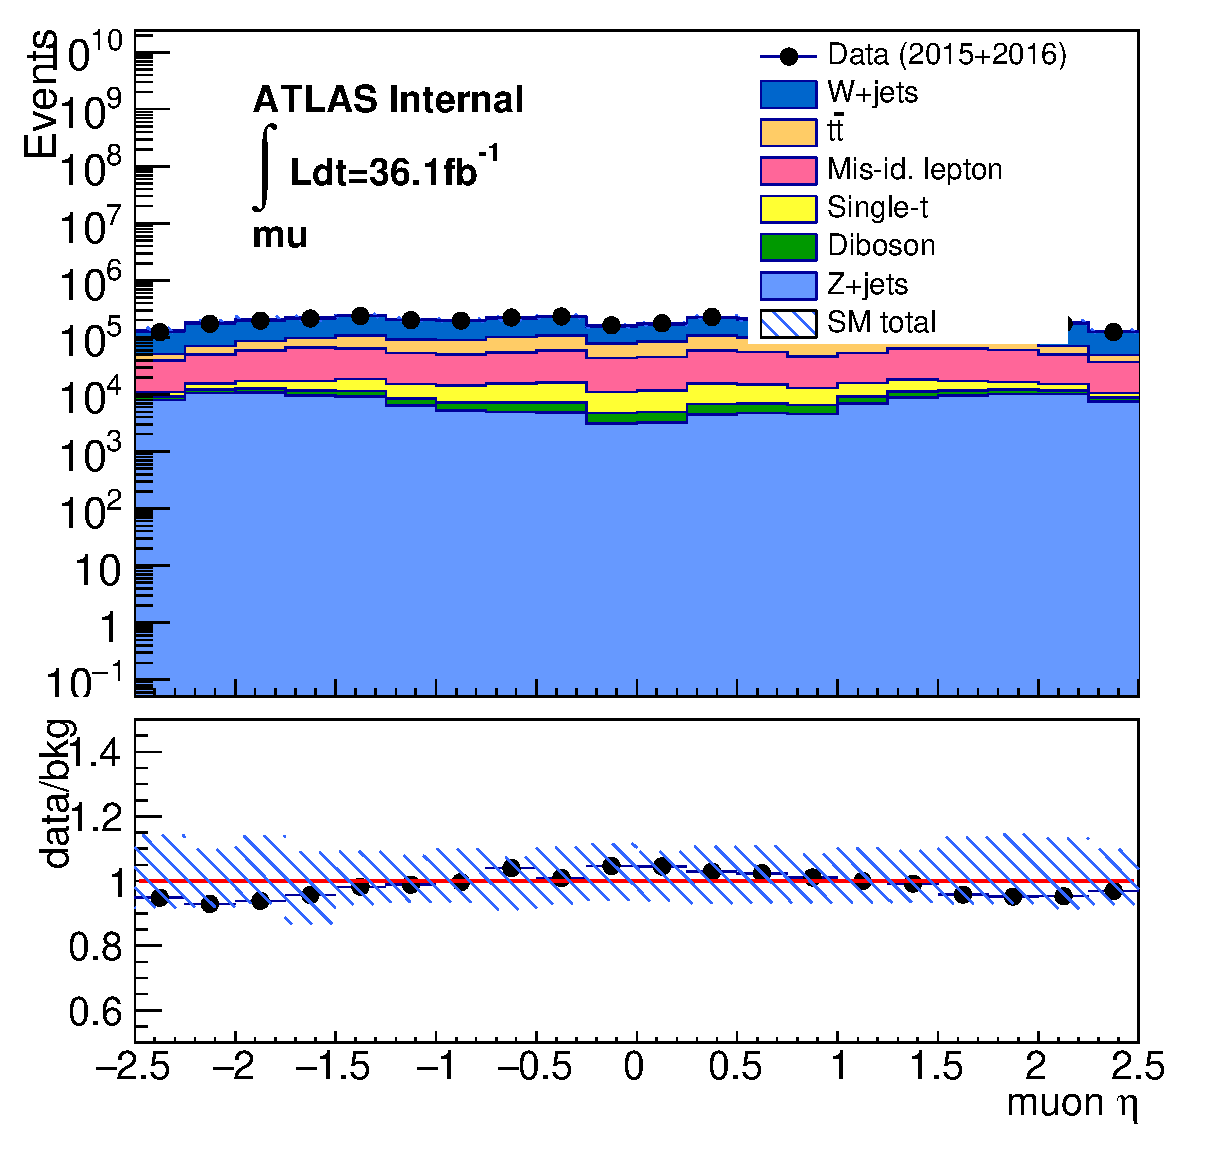
\includegraphics[width=0.43\textwidth]{Chapter3/MJ_VR/lep1eta_Loose_mu_lowWpt.eps}}\\
	\subfloat[]{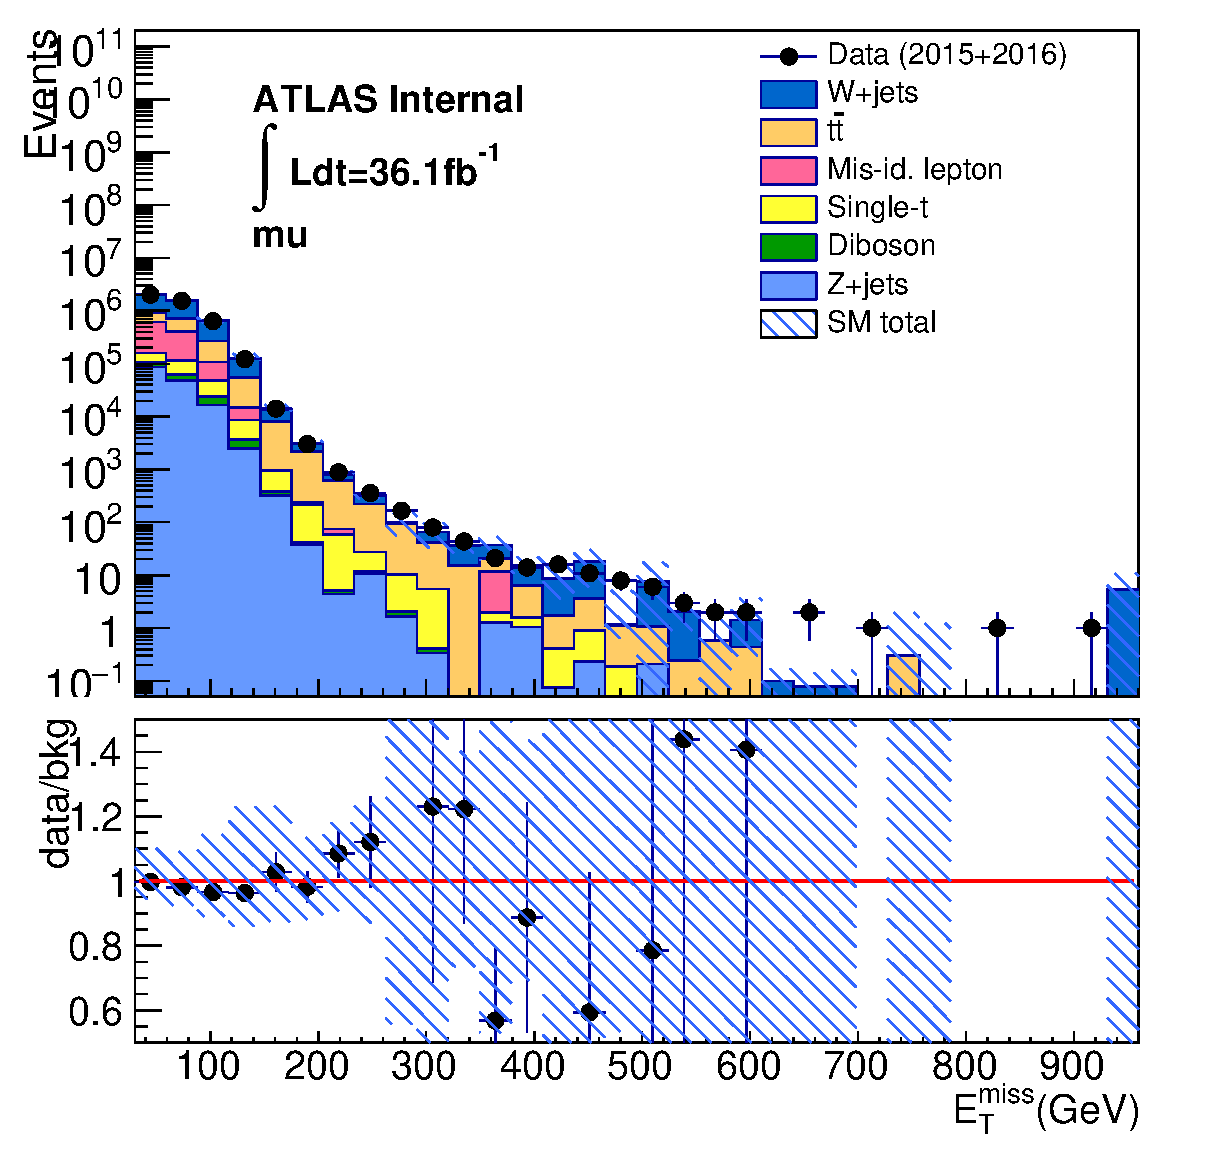
\includegraphics[width=0.43\textwidth]{Chapter3/MJ_VR/met_Loose_mu_lowWpt.eps}}
	\subfloat[]{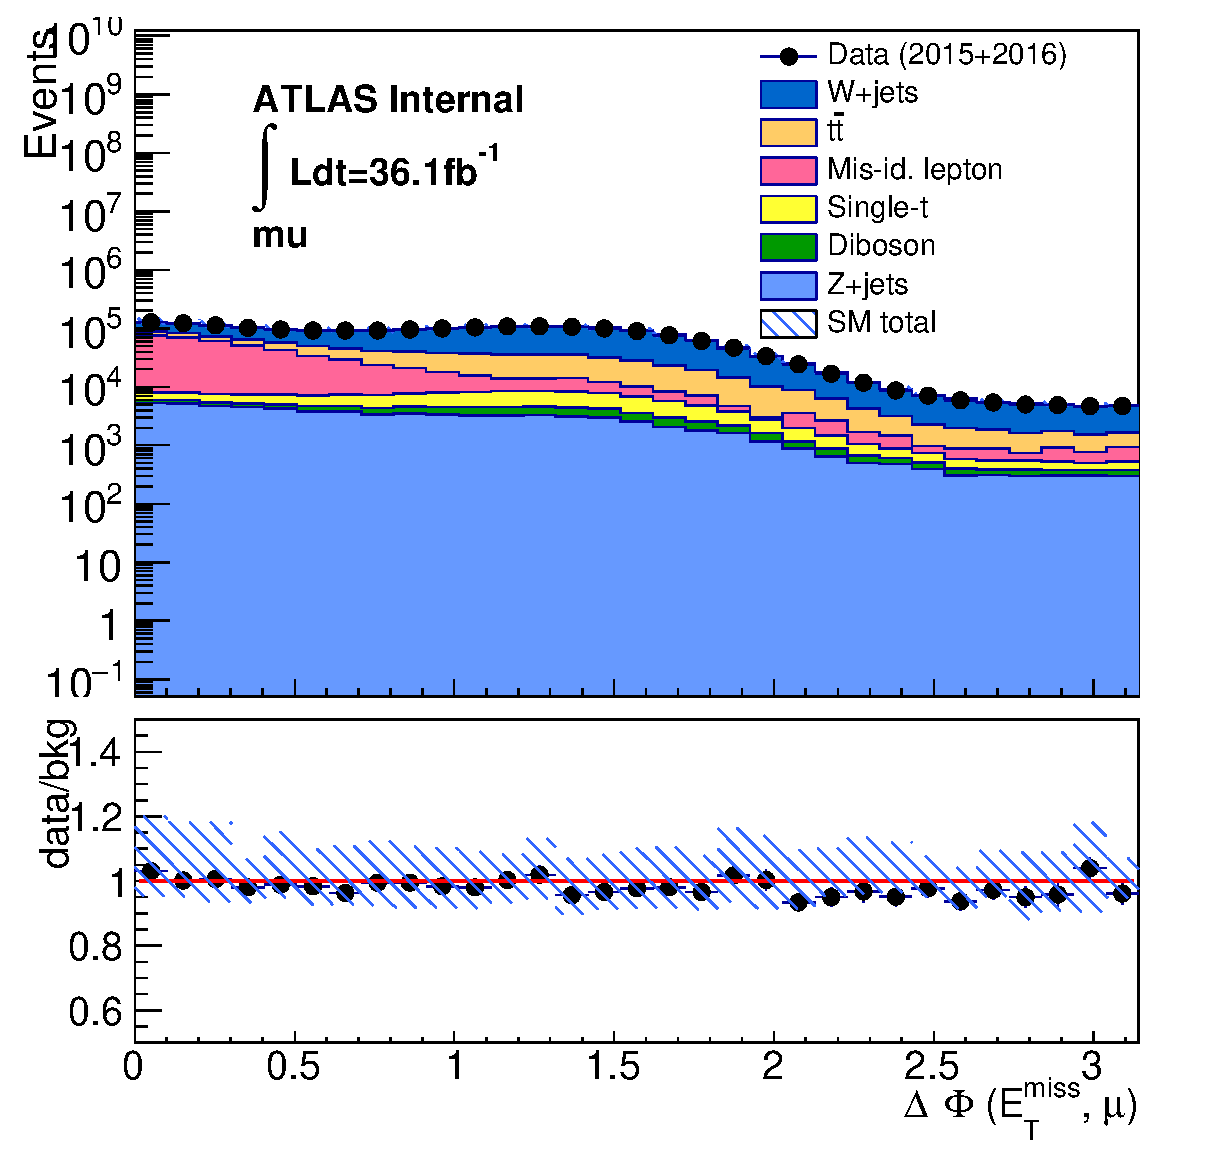
\includegraphics[width=0.43\textwidth]{Chapter3/MJ_VR/dphilepmet_Loose_mu_lowWpt.eps}}\\
	\subfloat[]{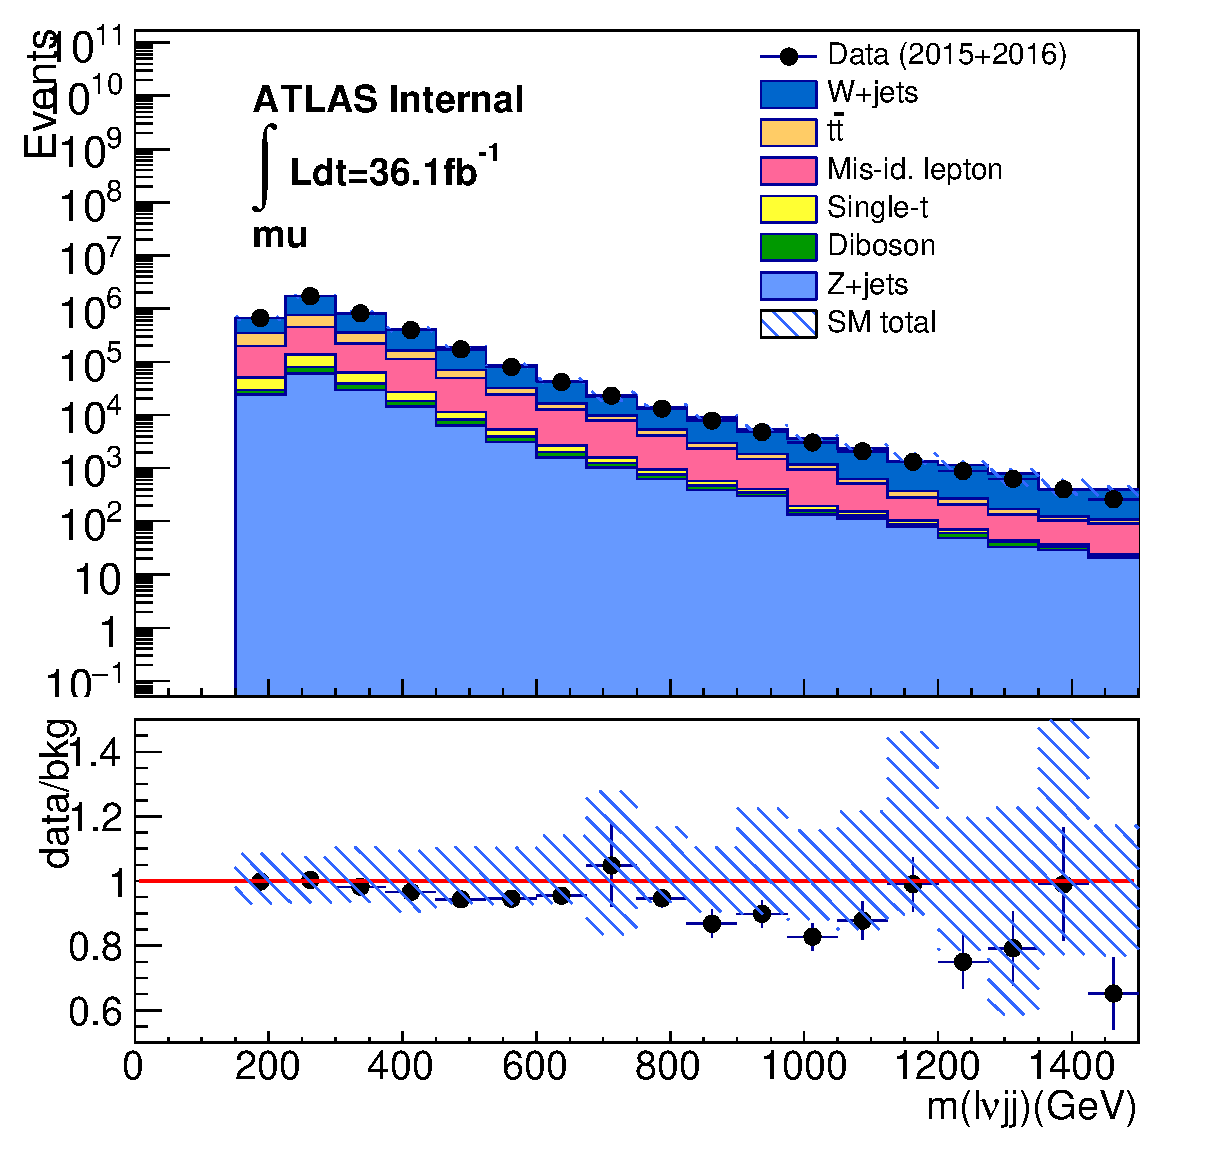
\includegraphics[width=0.43\textwidth]{Chapter3/MJ_VR/lvjjmass_Loose_mu_lowWpt.eps}}
	\caption{The distribution of lepton $p_{T}$, $\eta$, $E_{T}^{miss}$, $\Delta\phi$($\ell$,$E_{T}^{miss}$), and $m_{WV}$ in validation region with $p_{T}(l\nu)<150 GeV$ in muon channel with multijet background}
	\label{fig:FakeVR2_mu}
\end{figure}

\section{Data Background Comparison}
\label{Sec:data_bkg_compar}
To verify the modelling of background estimation, the data-MC comparison in top and W+jet control regions are performed for both VBF and ggF categories. The consistency is not perfect, as expected, since the fitting in the control regions exists to correct it as discussed in next chapter. The other issue in the background simulation is that a slope in the ratio of data over background is observed in $m^{VBF}$ distribution in VBF category for V+jet samples from Sherpa generator (it could be clearly seen in (d) of Fig.~\ref{Fig:mJJVBFWR}). In this analysis, it is also taken as one systematic uncertainty contribution to the simulation mismodelling. (Further discussion about this issue will be in Chap.~\ref{chap:VBFStrategy}.)
\\
\\Fig. \ref{Fig:ggFWR} and Fig. \ref{Fig:ggFTR} are the comparison plots for $m_{WV}$ in ggF category, while Fig. \ref{Fig:mWVVBFWR} to Fig. \ref{Fig:mWVVBFTR} are for VBF category. The comparison of  $m^{VBF}$ could be found in Fig. \ref{Fig:mJJVBFWR} and Fig. \ref{Fig:mJJVBFTR} to examine the VBF modelling. 
\newpage

\begin{figure}[ht]
	\centering
	\subfloat[]{\includegraphics[width=0.43\textwidth]{Chapter3/HighPurityCR_36fb/VVM_3_el}}
	\subfloat[]{\includegraphics[width=0.43\textwidth]{Chapter3/HighPurityCR_36fb/VVM_3_mu}}\\
	\subfloat[]{\includegraphics[width=0.43\textwidth]{Chapter3/LowPurityCR_36fb/VVM_12_el}}
	\subfloat[]{\includegraphics[width=0.43\textwidth]{Chapter3/LowPurityCR_36fb/VVM_12_mu}}\\
    \subfloat[]{\includegraphics[width=0.43\textwidth]{Chapter3/ResolvedCR/ggF36fb/VVM_5_el}}
	\subfloat[]{\includegraphics[width=0.43\textwidth]{Chapter3/ResolvedCR/ggF36fb/VVM_5_mu.eps}}
	\caption{The distribution of $m_{WV}$ in ggF high purity (top), low purity (middle), and resolved (bottom) W+jet control region for electron (left) and muon (right) channels respectively}
	\label{Fig:ggFWR}
\end{figure}



\begin{figure}[ht]
	\centering
	\subfloat[]{\includegraphics[width=0.43\textwidth]{Chapter3/HighPurityCR_36fb/VVM_2_el}}
	\subfloat[]{\includegraphics[width=0.43\textwidth]{Chapter3/HighPurityCR_36fb/VVM_2_mu}}\\
	\subfloat[]{\includegraphics[width=0.43\textwidth]{Chapter3/LowPurityCR_36fb/VVM_13_el}}
    \subfloat[]{\includegraphics[width=0.43\textwidth]{Chapter3/LowPurityCR_36fb/VVM_13_mu}}\\
	\subfloat[]{\includegraphics[width=0.43\textwidth]{Chapter3/ResolvedCR/ggF36fb/VVM_6_el}}
    \subfloat[]{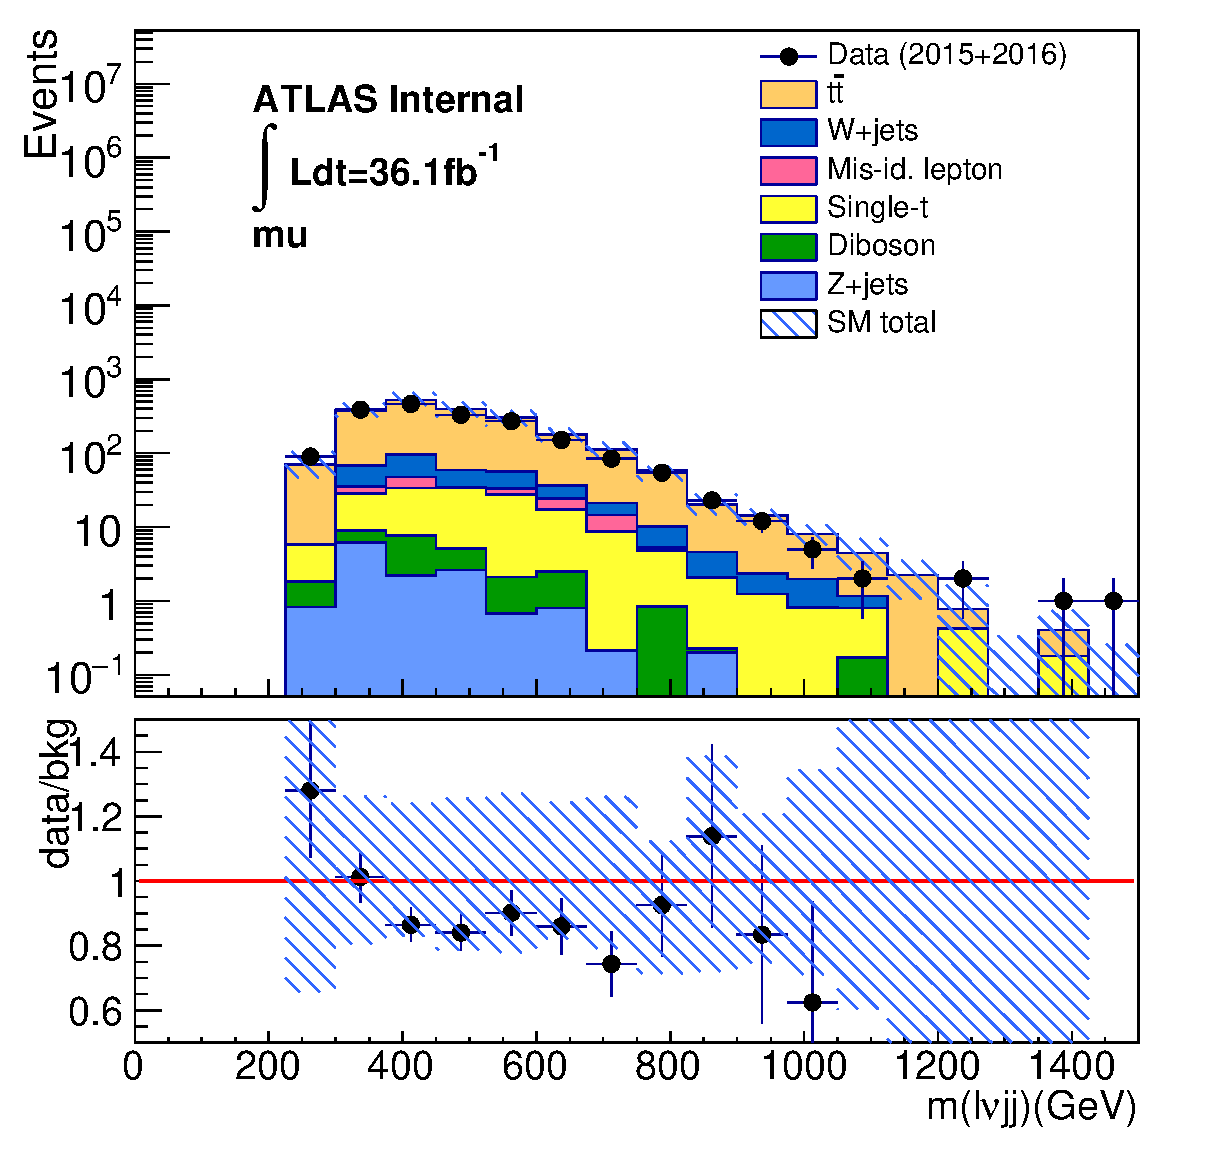
\includegraphics[width=0.43\textwidth]{Chapter3/ResolvedCR/ggF36fb/VVM_6_mu.eps}}
	\caption{The distribution of $m_{WV}$ in ggF high purity (top), low purity (middle), and resolved (bottom) top control region for electron (left) and muon (right) channels respectively}
	 \label{Fig:ggFTR}
\end{figure}


\begin{figure}[ht]
	\centering
	\subfloat[]{\includegraphics[width=0.43\textwidth]{Chapter3/VBF36fbHP/VVM_3_el}}
	\subfloat[]{\includegraphics[width=0.43\textwidth]{Chapter3/VBF36fbHP/VVM_3_mu}}\\
	\subfloat[]{\includegraphics[width=0.43\textwidth]{Chapter3/VBF36fbLP/VVM_12_el}}
    \subfloat[]{\includegraphics[width=0.43\textwidth]{Chapter3/VBF36fbLP/VVM_12_mu}}\\	
	\subfloat[]{\includegraphics[width=0.43\textwidth]{Chapter3/ResolvedCR/VBF36fb/VVM_5_el}}
    \subfloat[]{\includegraphics[width=0.43\textwidth]{Chapter3/ResolvedCR/VBF36fb/VVM_5_mu.eps}}    
	\caption{The distribution of $m_{WV}$ in VBF high purity (top), low purity (middle), and resolved (bottom) W+jet control region for electron (left) and muon (right) channels respectively}
	\label{Fig:mWVVBFWR}
\end{figure}
\clearpage
\begin{figure}[ht]
	\centering

	\subfloat[]{\includegraphics[width=0.43\textwidth]{Chapter3/VBF36fbHP/VBFmass_3_el}}
	\subfloat[]{\includegraphics[width=0.43\textwidth]{Chapter3/VBF36fbHP/VBFmass_3_mu}}\\
	\subfloat[]{\includegraphics[width=0.43\textwidth]{Chapter3/VBF36fbLP/VBFmass_12_el}}
    \subfloat[]{\includegraphics[width=0.43\textwidth]{Chapter3/VBF36fbLP/VBFmass_12_mu}}\\	
 	\subfloat[]{\includegraphics[width=0.43\textwidth]{Chapter3/ResolvedCR/VBF36fb/VBFmass_5_el}}
    \subfloat[]{\includegraphics[width=0.43\textwidth]{Chapter3/ResolvedCR/VBF36fb/VBFmass_5_mu}}\\   
	\caption{The distribution of $m^{VBF}$ in VBF high purity (top), low purity (middle), and resolved (bottom) W+jet control region for electron (left) and muon (right) channels respectively}
	\label{Fig:mJJVBFWR}
\end{figure}


\begin{figure}[ht]
	\centering
	\subfloat[]{\includegraphics[width=0.43\textwidth]{Chapter3/VBF36fbHP/VVM_2_el}}
	\subfloat[]{\includegraphics[width=0.43\textwidth]{Chapter3/VBF36fbHP/VVM_2_mu}}\\
	\subfloat[]{\includegraphics[width=0.43\textwidth]{Chapter3/VBF36fbLP/VVM_13_el}}
    \subfloat[]{\includegraphics[width=0.43\textwidth]{Chapter3/VBF36fbLP/VVM_13_mu}}\\
	\subfloat[]{\includegraphics[width=0.43\textwidth]{Chapter3/ResolvedCR/VBF36fb/VVM_6_el}}
    \subfloat[]{\includegraphics[width=0.43\textwidth]{Chapter3/ResolvedCR/VBF36fb/VVM_6_mu.eps}}	
	\caption{The distribution of $m_{WV}$ in VBF high purity (top), low purity (middle), and resolved (bottom) top control region for electron (left) and muon (right) channels respectively}
	\label{Fig:mWVVBFTR}
\end{figure}
\clearpage
\begin{figure}[ht]
	\centering
	\subfloat[]{\includegraphics[width=0.43\textwidth]{Chapter3/VBF36fbHP/VBFmass_2_el}}
	\subfloat[]{\includegraphics[width=0.43\textwidth]{Chapter3/VBF36fbHP/VBFmass_2_mu}}\\
	\subfloat[]{\includegraphics[width=0.43\textwidth]{Chapter3/VBF36fbLP/VBFmass_13_el}}
    \subfloat[]{\includegraphics[width=0.43\textwidth]{Chapter3/VBF36fbLP/VBFmass_13_mu}}\\	
    \subfloat[]{\includegraphics[width=0.43\textwidth]{Chapter3/ResolvedCR/VBF36fb/VBFmass_6_el}}
    \subfloat[]{\includegraphics[width=0.43\textwidth]{Chapter3/ResolvedCR/VBF36fb/VBFmass_6_mu}}\\
	\caption{The distribution of $m^{VBF}$ in VBF high purity (top), low purity (middle), and resolved (bottom) top control region for electron (left) and muon (right) channels respectivelyy}
	\label{Fig:mJJVBFTR}
\end{figure}

